This section presents the definitions of the objects used in the analysis: jets, electrons, muons and $\met$. 
%Unless otherwise stated, the recommendations implemented in SUSYTools-00-05-06-23-03 tag and analysis release SUSY,2.3.24a 
Unless otherwise stated, the recommendations implemented in SUSYTools-00-07-17 tag and analysis release SUSY,2.3.38b 
are used for all the objects; most of the studies that led to these definitions were however performed with earlier tags. 
Note that the electron identification scale factors released on 15/01/16 within the ElectronEfficiencyCorrection-00-01-39 
package are used for AtlFast2 samples in the final results since they differ by up to 10\% in the barrel region with respect 
to those included in analysis release SUSY,2.3.38b.

\subsection{Jets}
\label{sec:objects_jets}

The jet selection is summarized in Table~\ref{tab:jetsdef}. 
Jets are reconstructed using the anti-$k_{t}$ jet algorithm~\cite{Cacciari:2008gp} 
with the distance parameter $R$ set to $0.4$ and topological clusters as input. 
Jets are calibrated with the EMTopo scheme applying the jet area pile up corrections. 
The jets are kept only if they have $p_\mathrm{T}>20$~GeV and lie within $|\eta|<2.8$. 
To mitigate the effects of pileup, Jet Vertex Tagger ({\sc JVT})~\cite{ATLAS-CONF-2014-018} requirements 
are applied to the selected jets as recommended by the JetEtMiss group (reject jets after the overlap removal procedure with $\pt<50$~GeV, $|\eta|<2.4$ and JVT$<$0.64). 
The gain in stability with respect to pile-up after
applying this set of cut is illustrated in Figure~\ref{Figure:JVF_Dependency_Run2}.
In order to remove events with fake \met, an event is vetoed 
when a jet ($|\eta|<4.9$) with quality judged as bad according to the {\tt VeryLoose} criterion is present. 

%%%%%%%%%%%%%%%%%%%%%%%%%%%%%%%%%%%%%%%%%%%%%%%%%%%%%%%%%%%%%
\begin{table}[htb!]
\caption{Summary of the jet selection criteria. }
\label{tab:jetsdef}
\begin{center}
    \begin{tabular}{|l|c|}
      \hline
      \hline
      \multicolumn{2}{|c|}{\textbf{Pre-selected jet}}\\
    \hline
      \hline
      Collection     & AntiKt4EMTopo \\
      \hline
      Acceptance     & $\pt > 20\,\GeV, |\eta | < 2.8$ \\
      \hline
      Overlap        & see section~\ref{sec:objects_overlap_removal} \\ % $\Delta{}R({\mathrm jet},e)$~$>$~0.2
\hline
 Jet vertex tagger  &  reject jets with $\pt<50$ GeV, $|\eta|<2.4$ \\
                    &   and JVT$<$0.64 after overlap removal\\
      \hline\hline
%      \multicolumn{2}{|c|}{\textbf{Signal jet}}\\
%      \hline
%     Acceptance     & $\pt > 40\,\GeV,$ \\
%      & $|\eta | < 2.8$ \\ 
%     \hline
%      \hline
      \multicolumn{2}{|c|}{\textbf{b-jets}}\\
    \hline
      \hline
     Acceptance     & $\pt > 20\,\GeV,$ \\
      & $|\eta | < 2.5$ \\ 
      \hline
   $b$-tagging  &  MV2c20 algorithm 70\% OP\\
                &  MV2c20 algorithm 80\% OP for overlap removal\\

      \hline   
\end{tabular}
\end{center}
\end{table}

\begin{figure}[h!]
\begin{center}
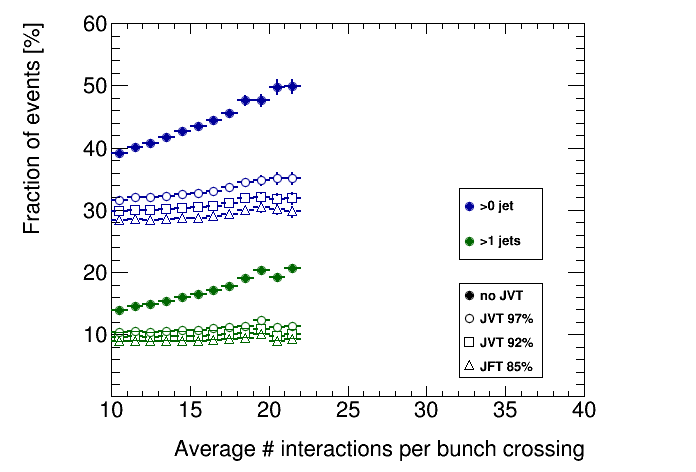
\includegraphics[trim=0.0cm 0cm 0cm 0cm,width=0.47\columnwidth]{FIGURES/Frac_njets_1and2}
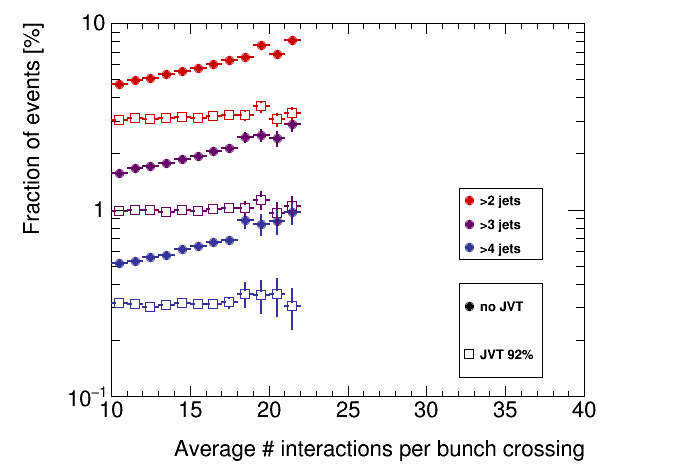
\includegraphics[trim=0.0cm 0cm 0cm 0cm,width=0.47\columnwidth]{FIGURES/Frac_njets_3to5}
\vspace{-0.2cm}
\end{center}
\caption{Fraction of events [\%] in data with at least 1 or 2 jets (left) and with at least 3, 4 or 5 jets (right) with respect to average number of interactions per bunch crossing with and without a cut on the JVT. Event selection requires a pair of leptons, and all jets have \pt~$>$~25\GeV. $L$~=~3.2~fb$^{-1}$ and $\sqrt s$~=~13\TeV.}
\label{Figure:JVF_Dependency_Run2} 
\end{figure}
%%%%%%%%%%%%%%%%%%%%%%%%%%%%%%%%%%%%%%%%%%%%%%%%%%%%%%%%%%%%

\subsubsection{$b$-tagging}

Tagging of $b$-jets is done using the MV2c20 algorithm with the 70\% efficiency 
operating point. This algorithm is based on a neural network using 
the output weights of the JetFitter+IP3D, IP3D and SV1 algorithms as input.
This efficiency working point was favored by optimisation studies performed with MC15 simulated signal and background samples as described below.
Figure~\ref{fig:btagging} shows the $b$-jet multiplicity for the three tagging efficiency working points. 
Monte Carlo background distributions are shown after same-sign lepton pair requirement.

\begin{figure}[htb!!]
\begin{center}
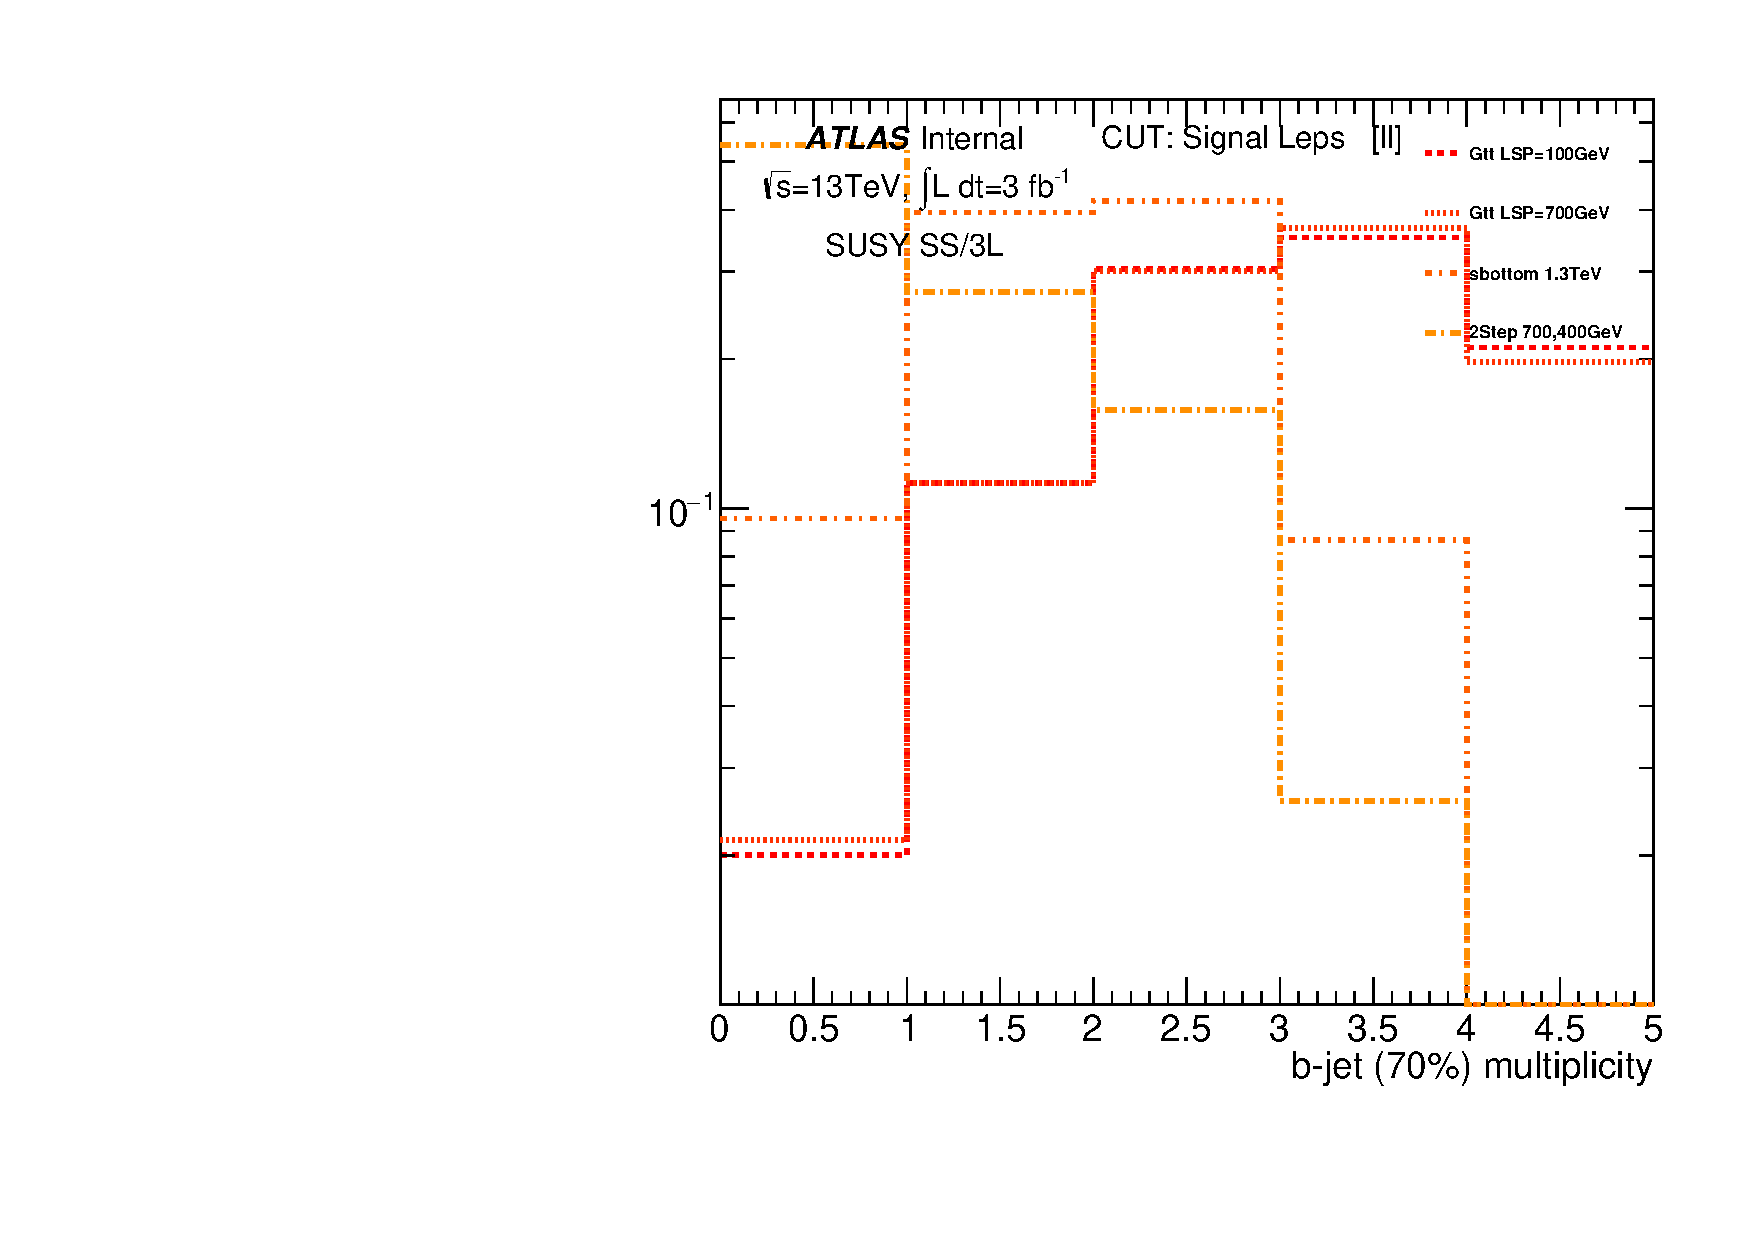
\includegraphics[width=0.3\textwidth]{FIGURES/BTAGGING/02_CutLEP_ll_NB1JET_signals.pdf} 
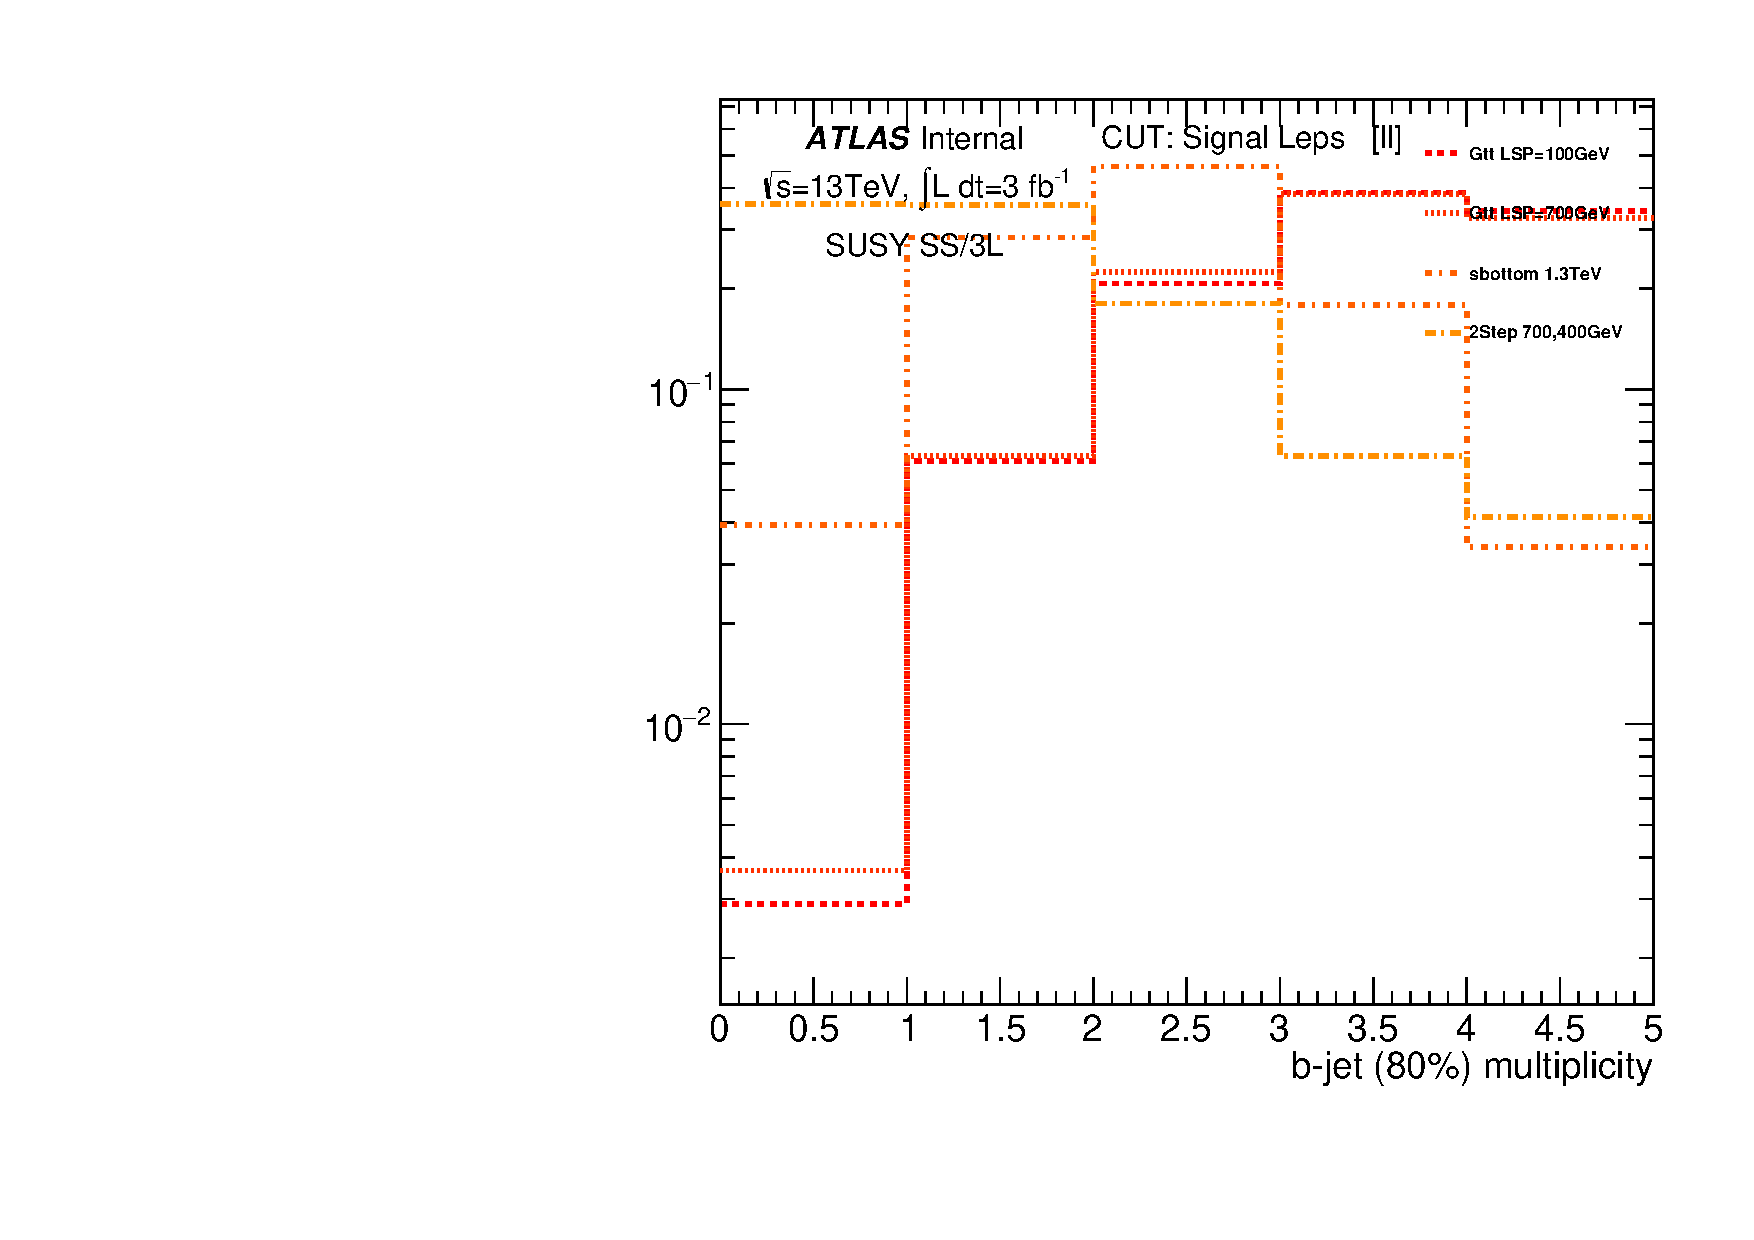
\includegraphics[width=0.3\textwidth]{FIGURES/BTAGGING/02_CutLEP_ll_NB2JET_signals.pdf}
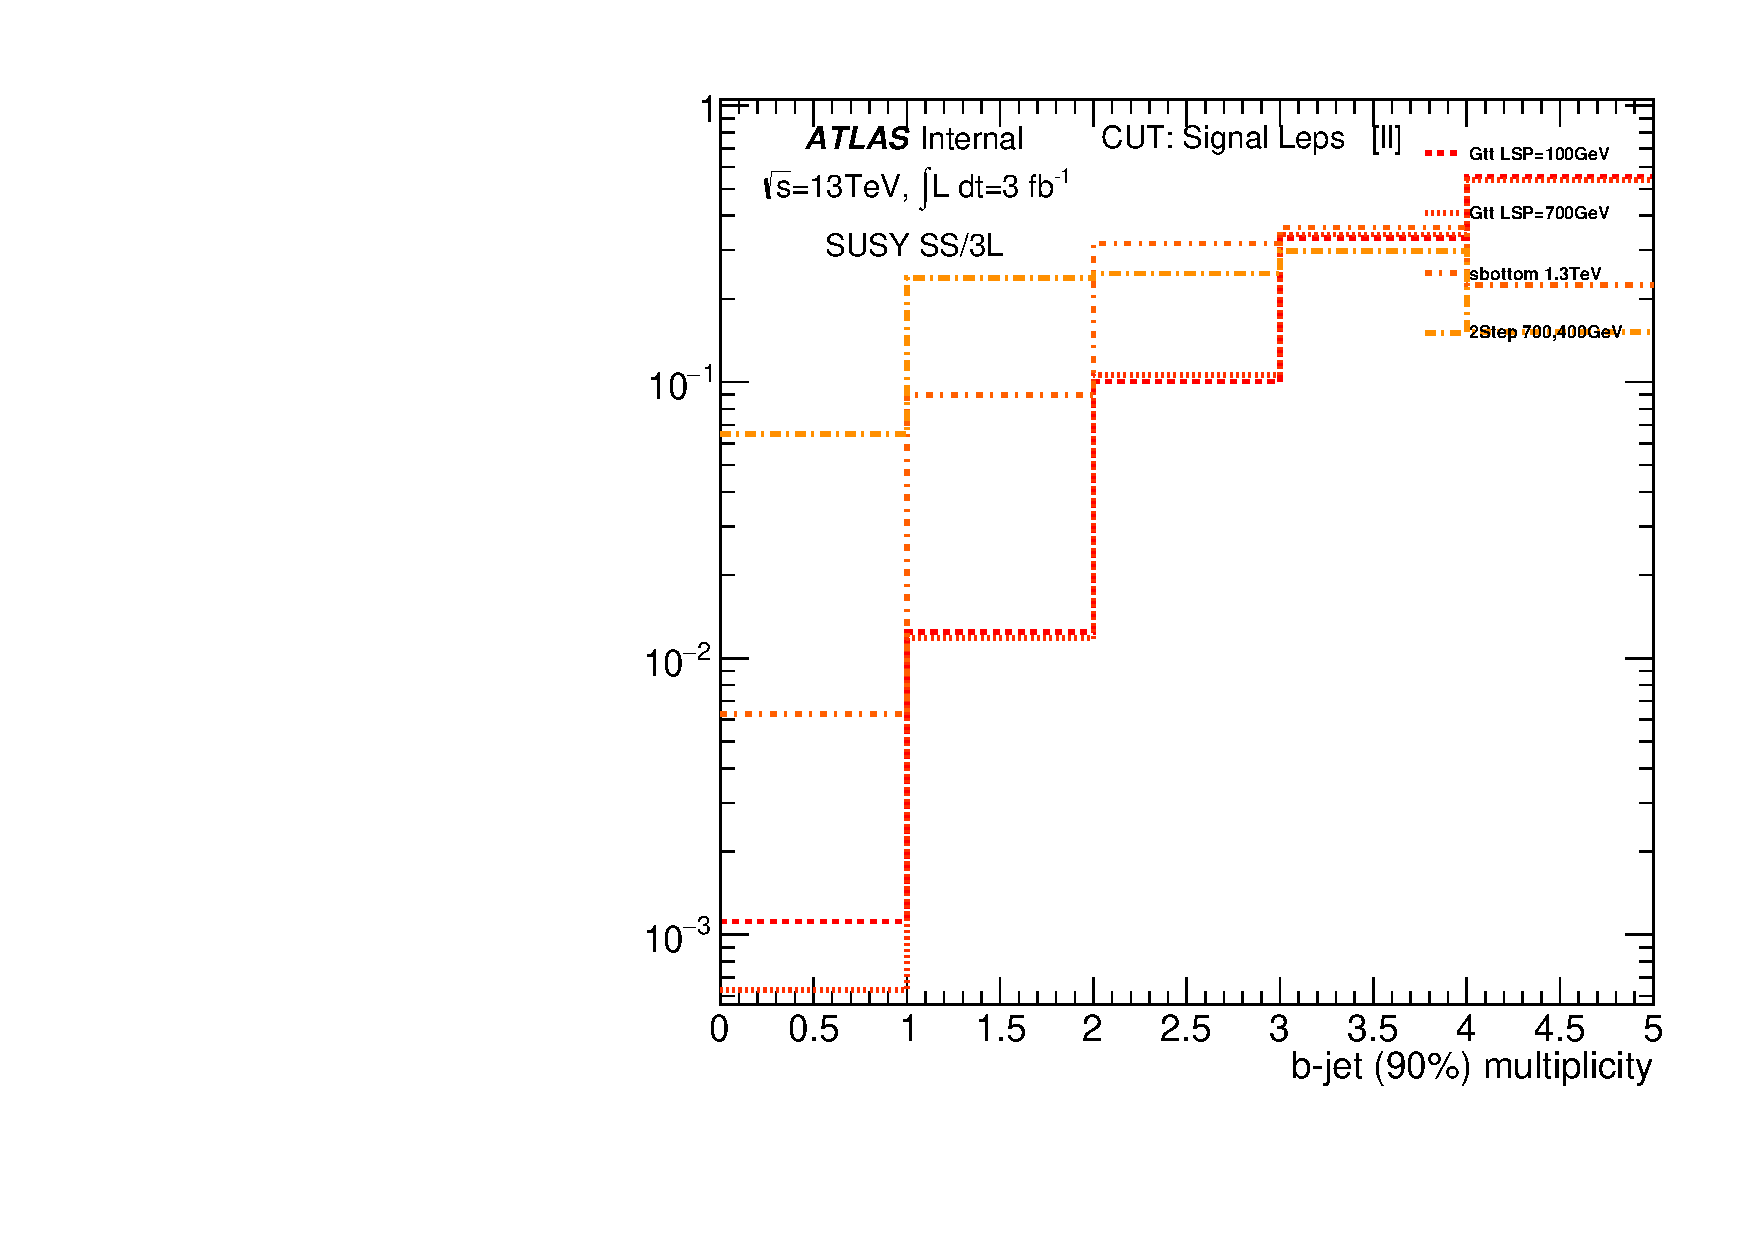
\includegraphics[width=0.3\textwidth]{FIGURES/BTAGGING/02_CutLEP_ll_NB3JET_signals.pdf}\\ 
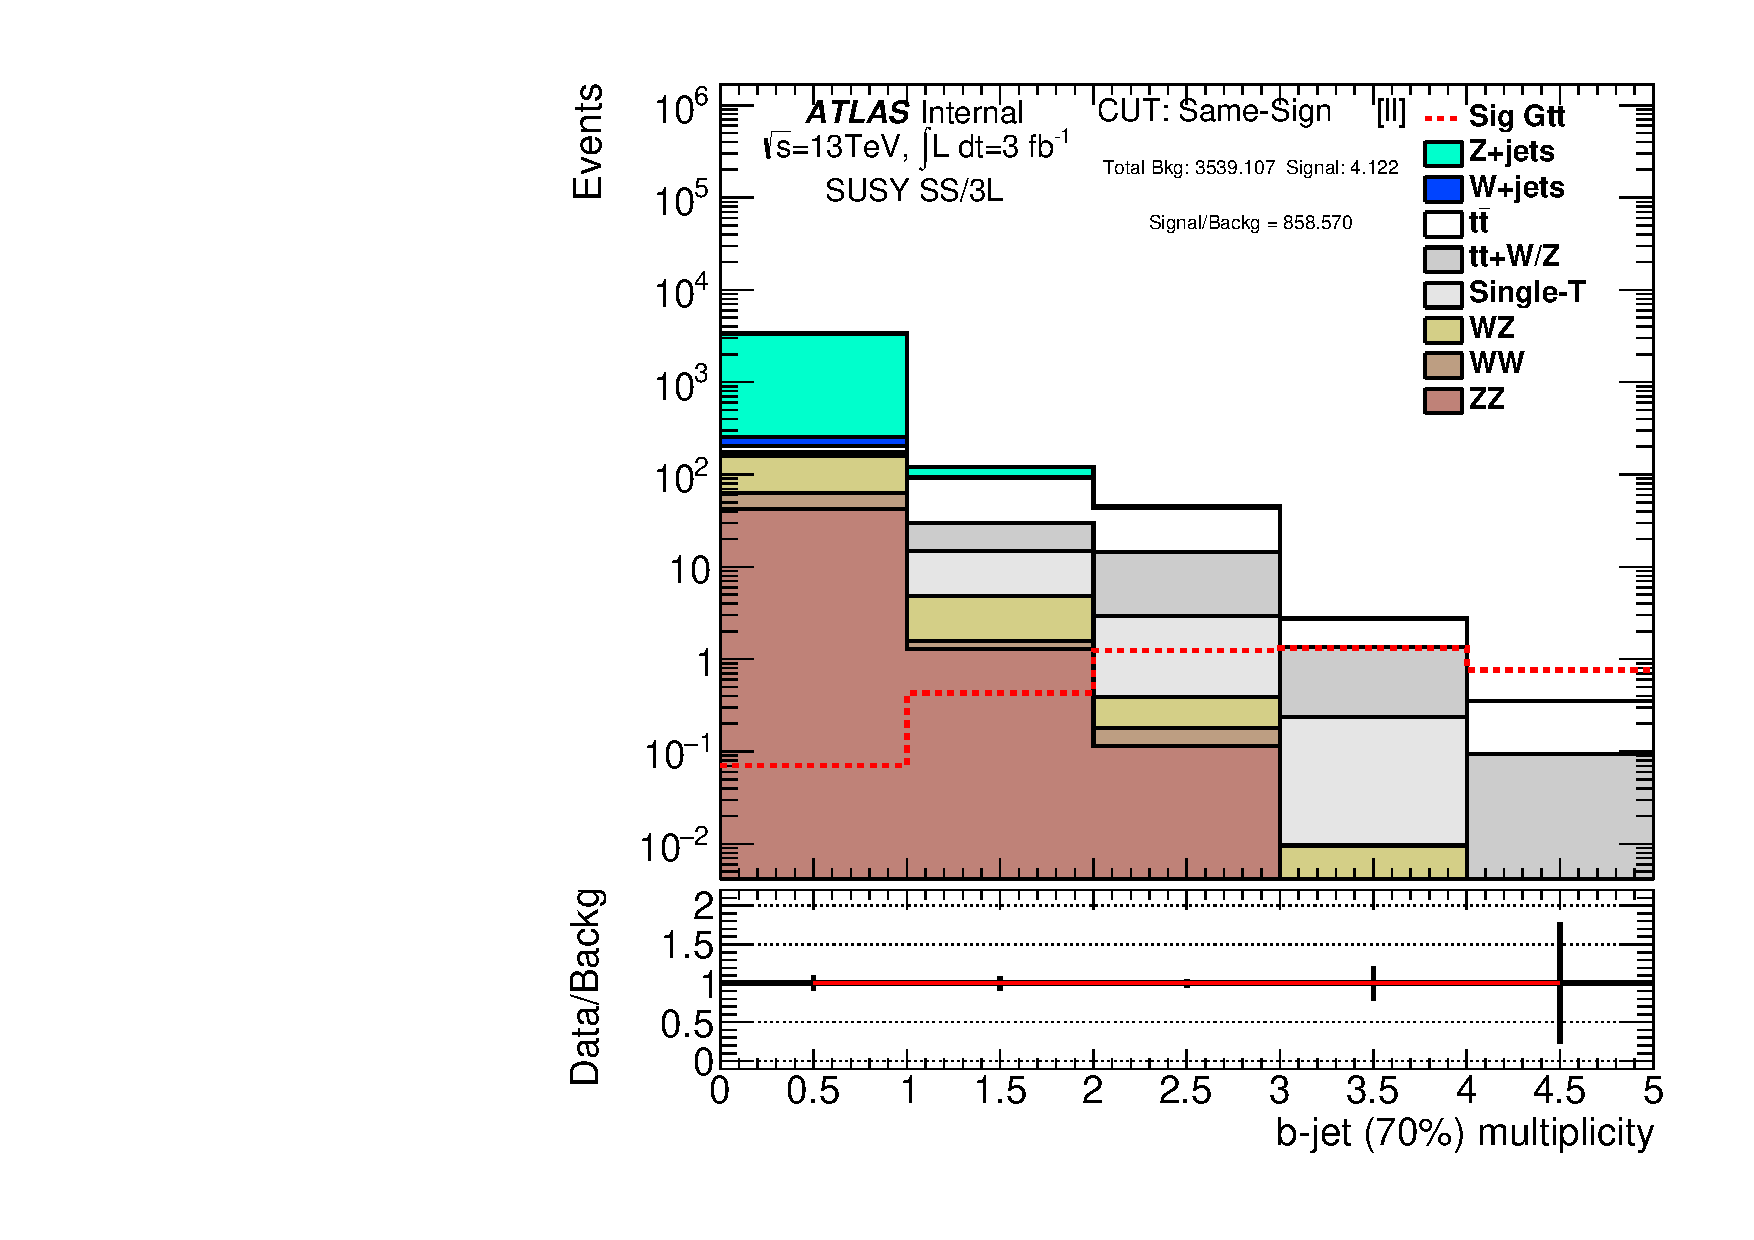
\includegraphics[width=0.3\textwidth]{FIGURES/BTAGGING/05_CutSS_ll_NB1JET.pdf}
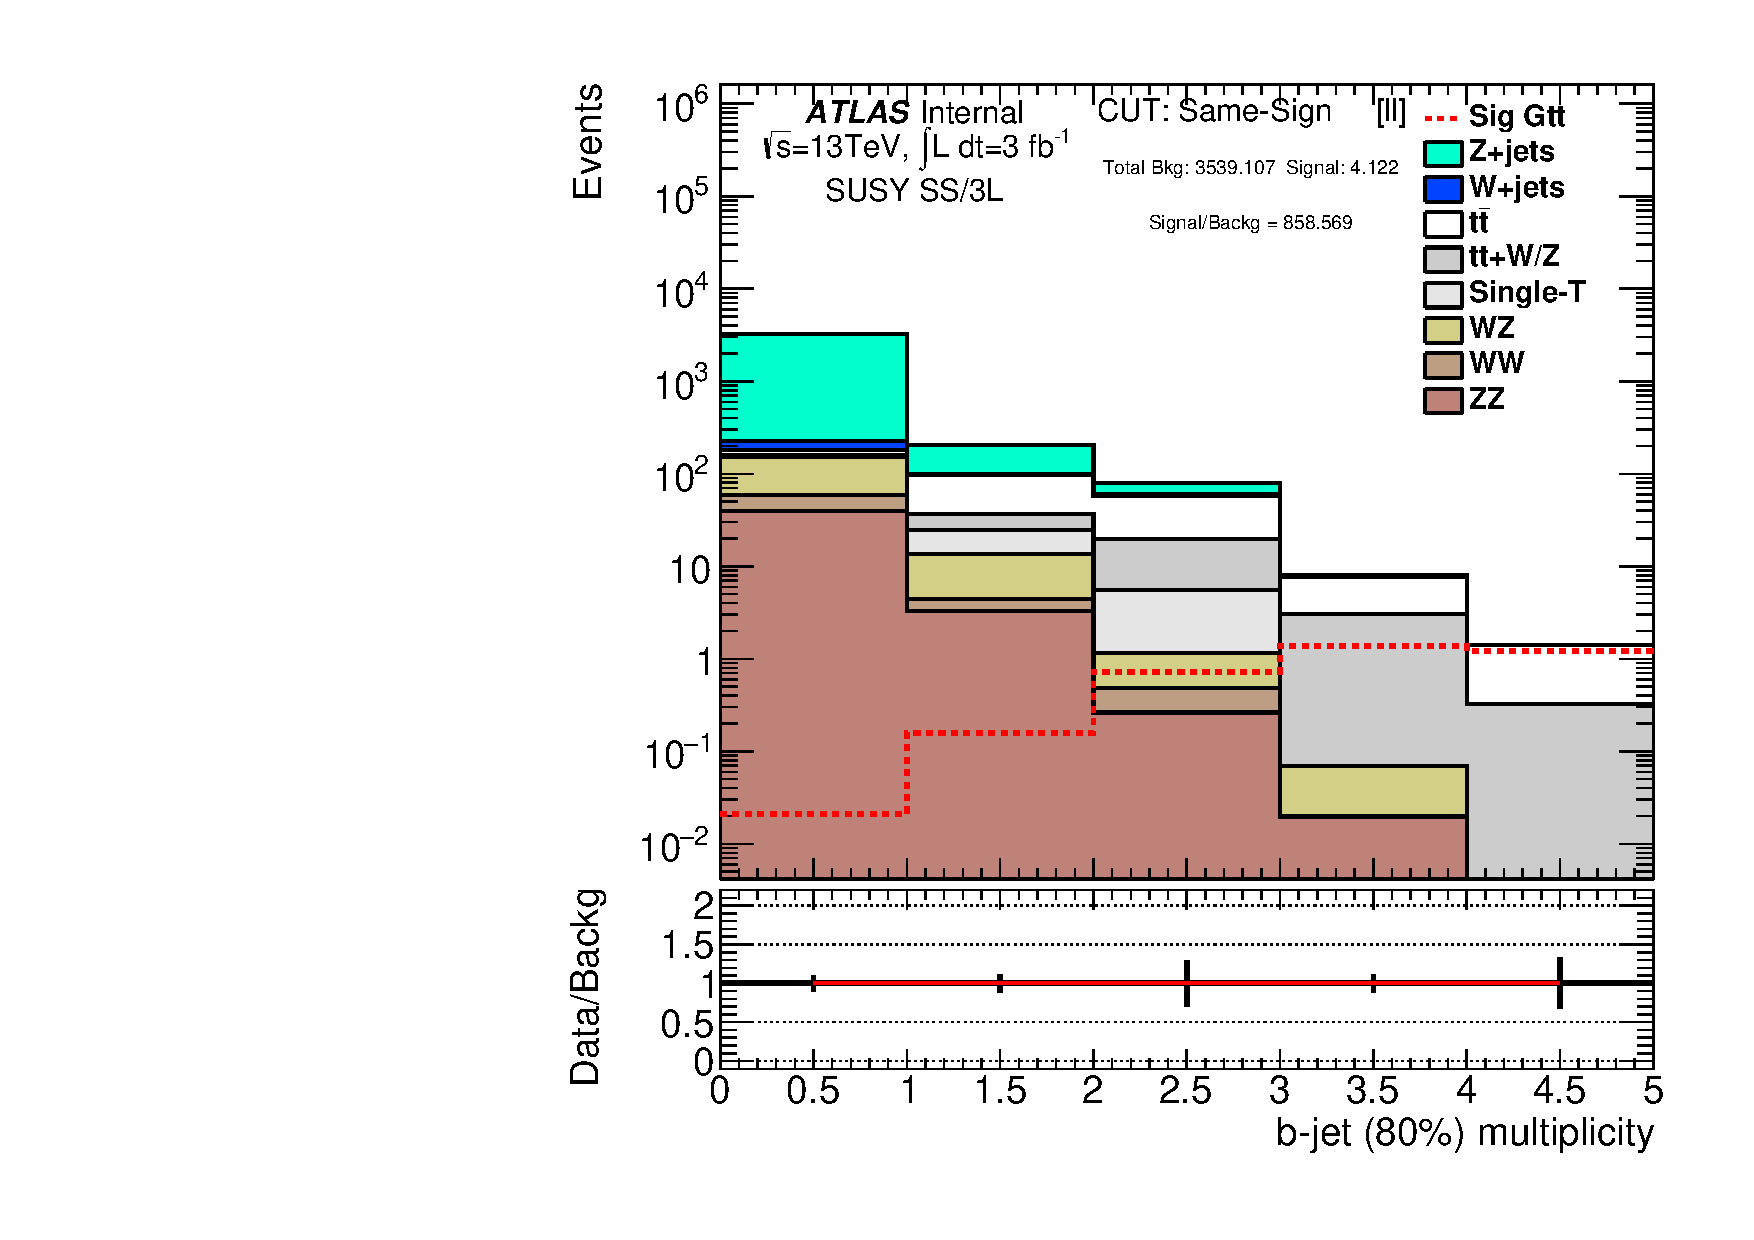
\includegraphics[width=0.3\textwidth]{FIGURES/BTAGGING/05_CutSS_ll_NB2JET.pdf}
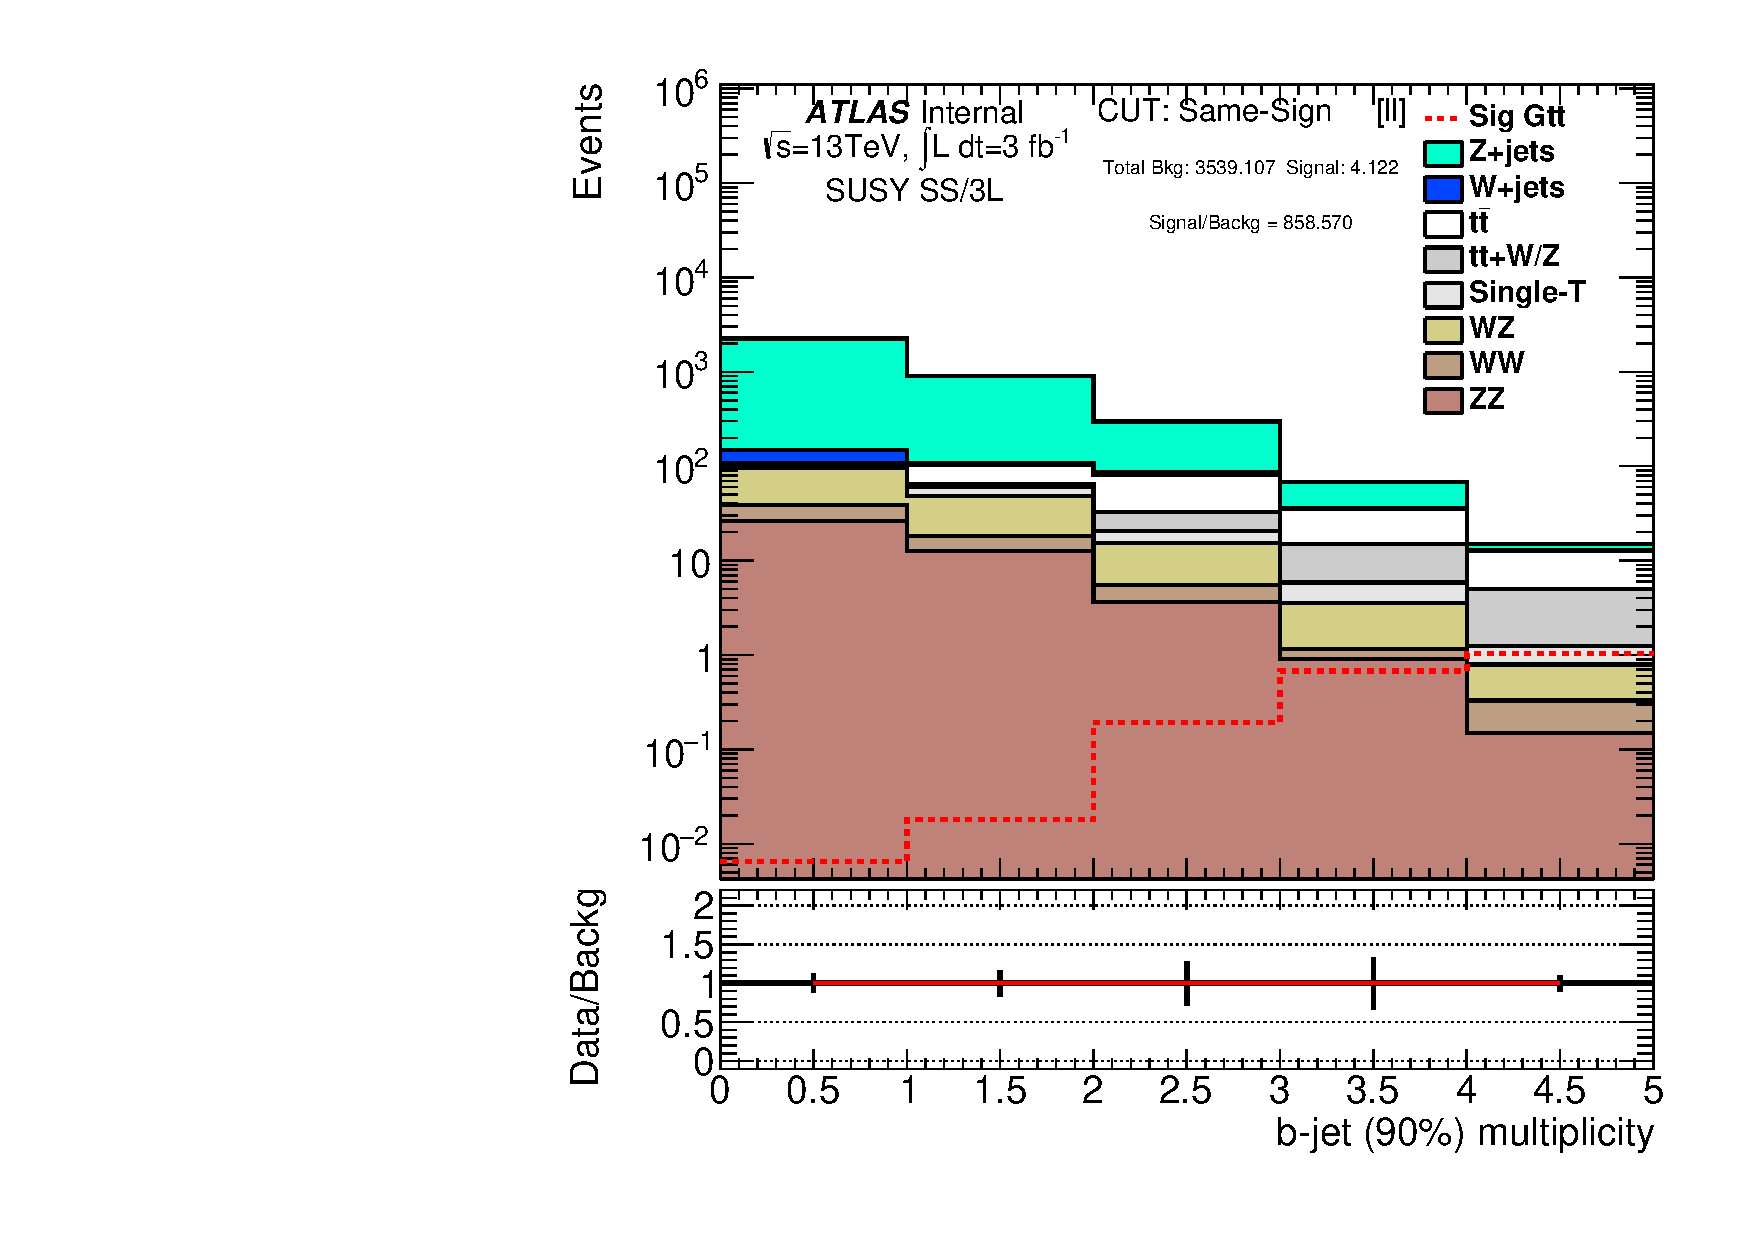
\includegraphics[width=0.3\textwidth]{FIGURES/BTAGGING/05_CutSS_ll_NB3JET.pdf} 
\end{center}
\vspace{-0.2cm}
\caption{$b$-jet multiplicity for three different tagging efficiency working points, left 70\%, center 80\%, right 90\%.
Signals shapes are shown on the top figures, and stacked background expectations for an integrated luminosity of 3~fb$^{-1}$ are shown on the bottom plots.}
\label{fig:btagging}
\end{figure}

Different signal models described earlier on this document are expected to contain different heavy flavour jet multiplicities.
Therefore the choice of the most performant $b$-jet tagging efficiency working point was made by looking into regions that emulate the signal regions that would eventually be used in the analysis.
Table~\ref{tab:btaggingSR} describes the six different signal-like regions used on this optimisation. 

%%%%%%%%%%%%%%%%%%%%%%%%%%%%%%%%%%%%%%%%%%%%%%%%%%%%%%%%%%%%%
\begin{table}[htb!]
\caption{Signal-like region selections used for the $b$-jet efficiency working point optimisation.}
\label{tab:btaggingSR}
\begin{center}
\begin{tabular}{l|c|c|l}
                & \#$\ell$ & \#$b$-jets & Other cuts                          \\ \hline \hline
  SR-3$b$       & $\geq 2$ & $\geq 3$   & $N^{40}_j \geq 6$                    \\
  SR-3$b$ Soft  & $\geq 2$ & $\geq 3$   & $N^{20}_j \geq 7$ \&\& MET$>$150~GeV \\\hline
  SR-1$b$       & $\geq 2$ & $\geq 1$   & $N^{50}_j \geq 4$ \&\& MET$>$150~GeV (!SR3b)\\
  SR-1$b$ Incl  & $\geq 2$ & $\geq 1$   & $N^{40}_j \geq 4$ \&\& MET$>$150~GeV \\\hline
  SR-0$b$- 5j   & $\geq 2$ & $== 0$     & $N^{50}_j \geq 5$ \&\& MET$>$100~GeV \\
  SR-0$b$- 3j   & $\geq 2$ & $== 0$     & $N^{40}_j \geq 3$ \&\& MET$>$200~GeV \\ \hline
\end{tabular}
\end{center}
\end{table}
%%%%%%%%%%%%%%%%%%%%%%%%%%%%%%%%%%%%%%%%%%%%%%%%%%%%%%%%%%%%
         
\begin{figure}[htb!!]
\begin{center}
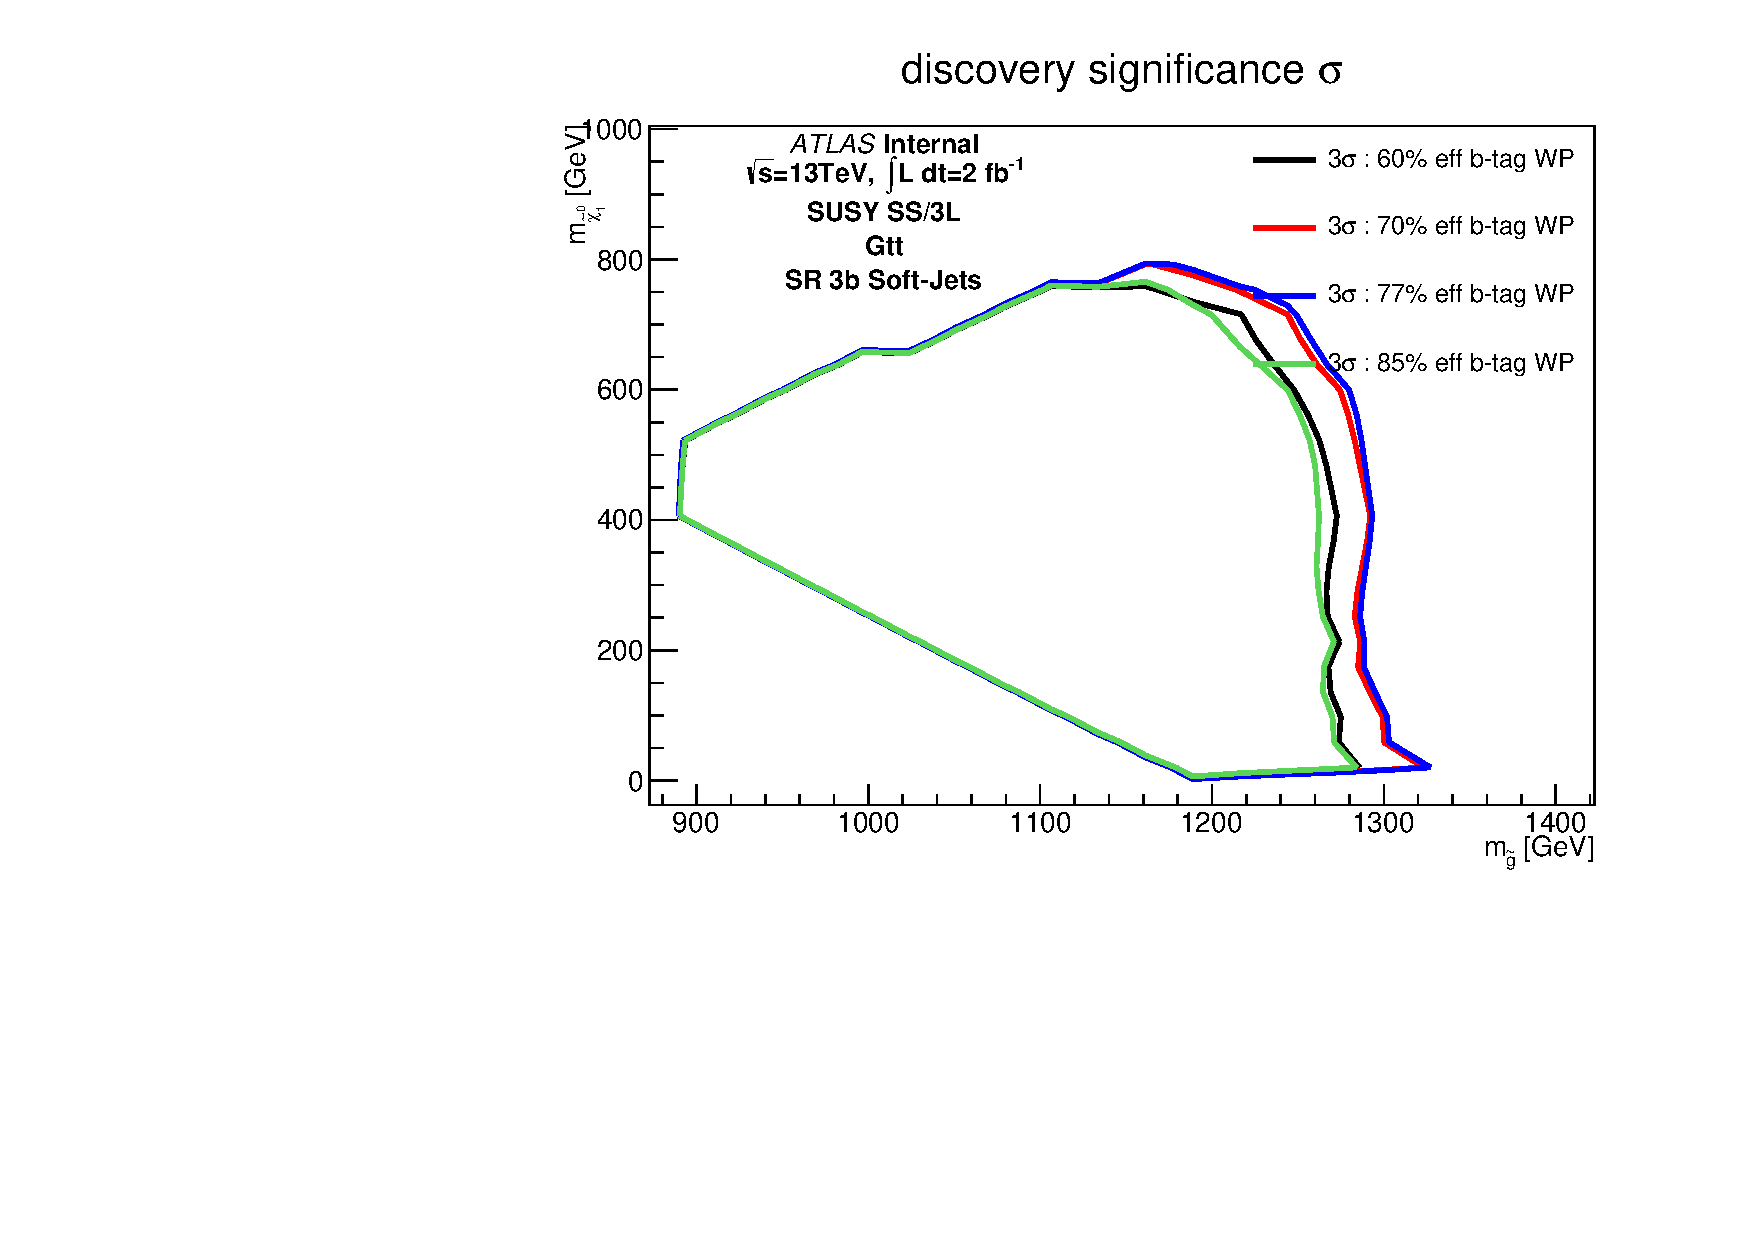
\includegraphics[width=0.45\textwidth]{FIGURES/BTAGGINGMC15/L2fb/plot_significance_gtt_CutSR3BS60_all.pdf}\\
%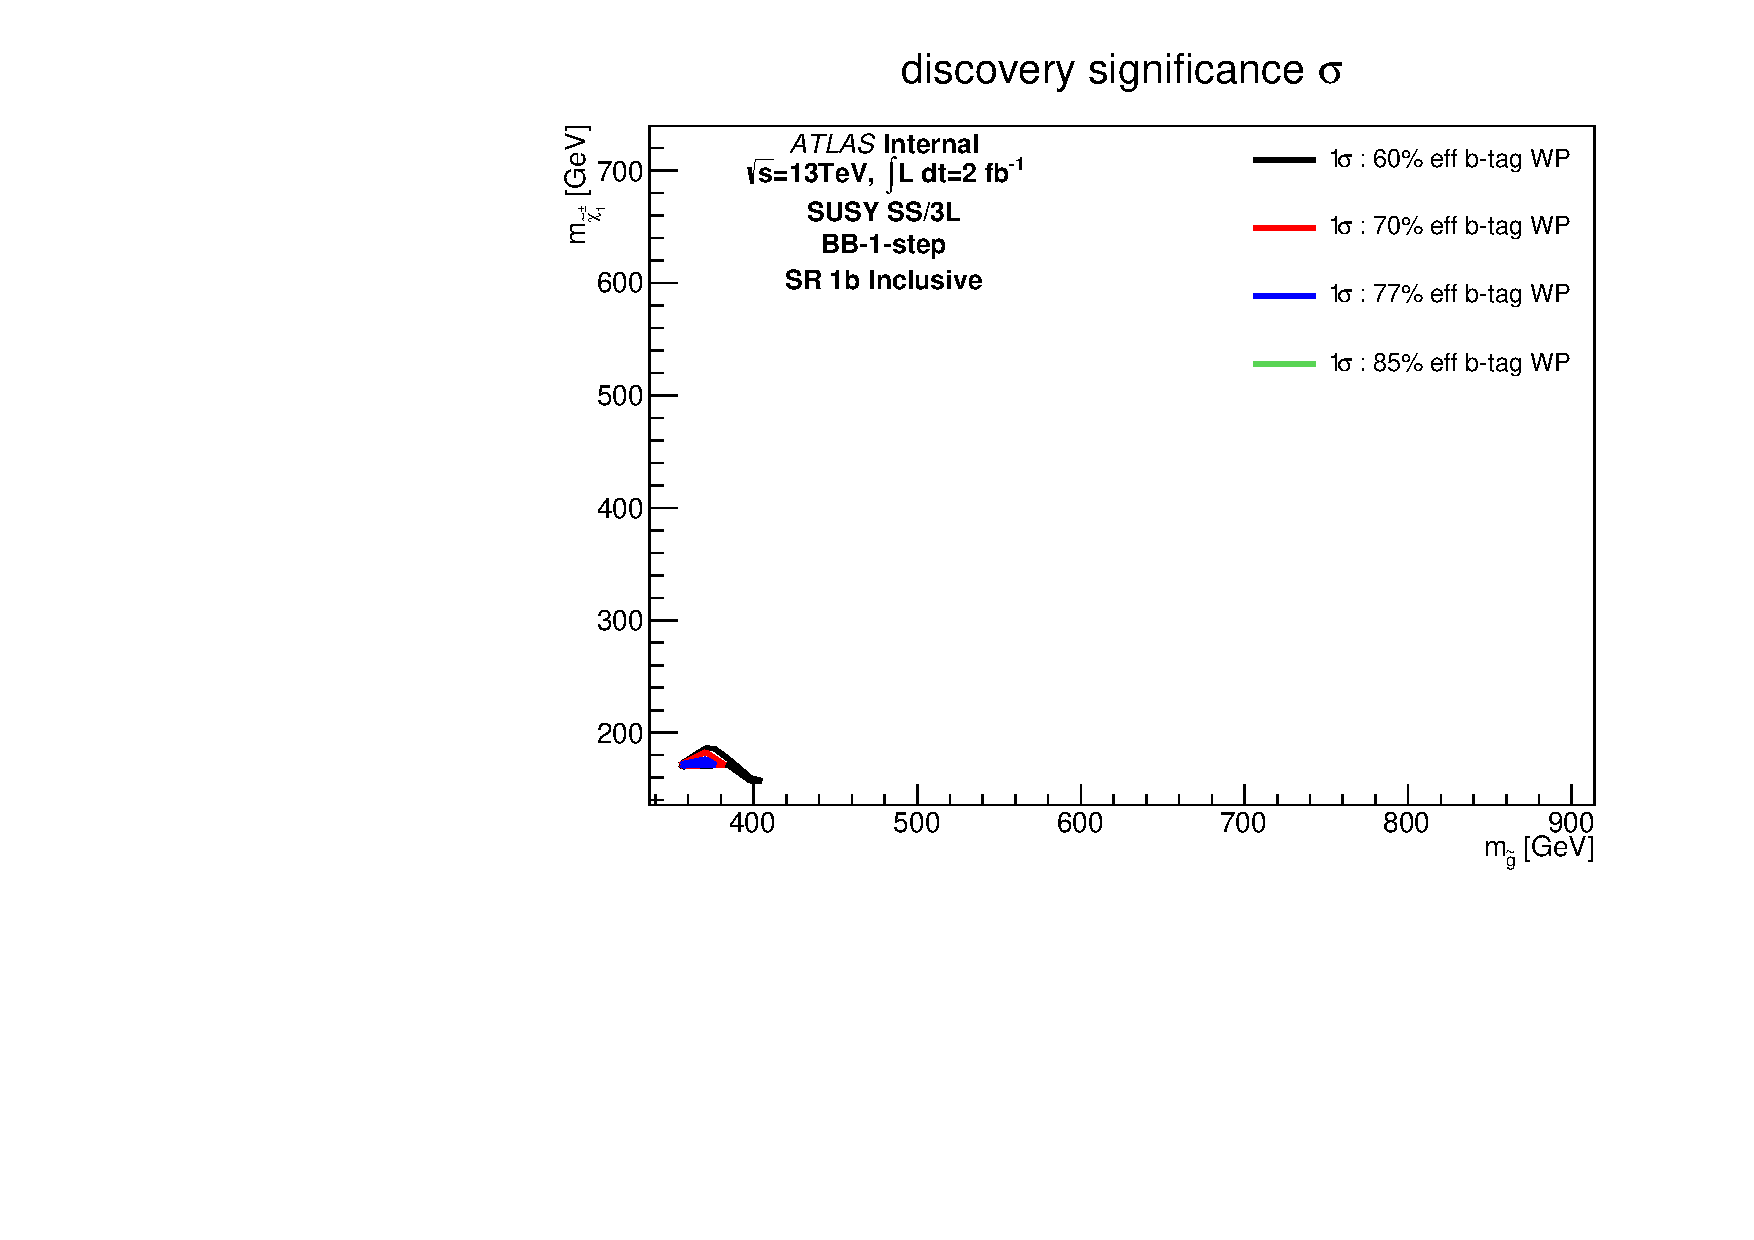
\includegraphics[width=0.3\textwidth]{FIGURES/BTAGGINGMC15/L2fb/plot_significance_bb1step_CutSR1BI60_all.pdf}\\
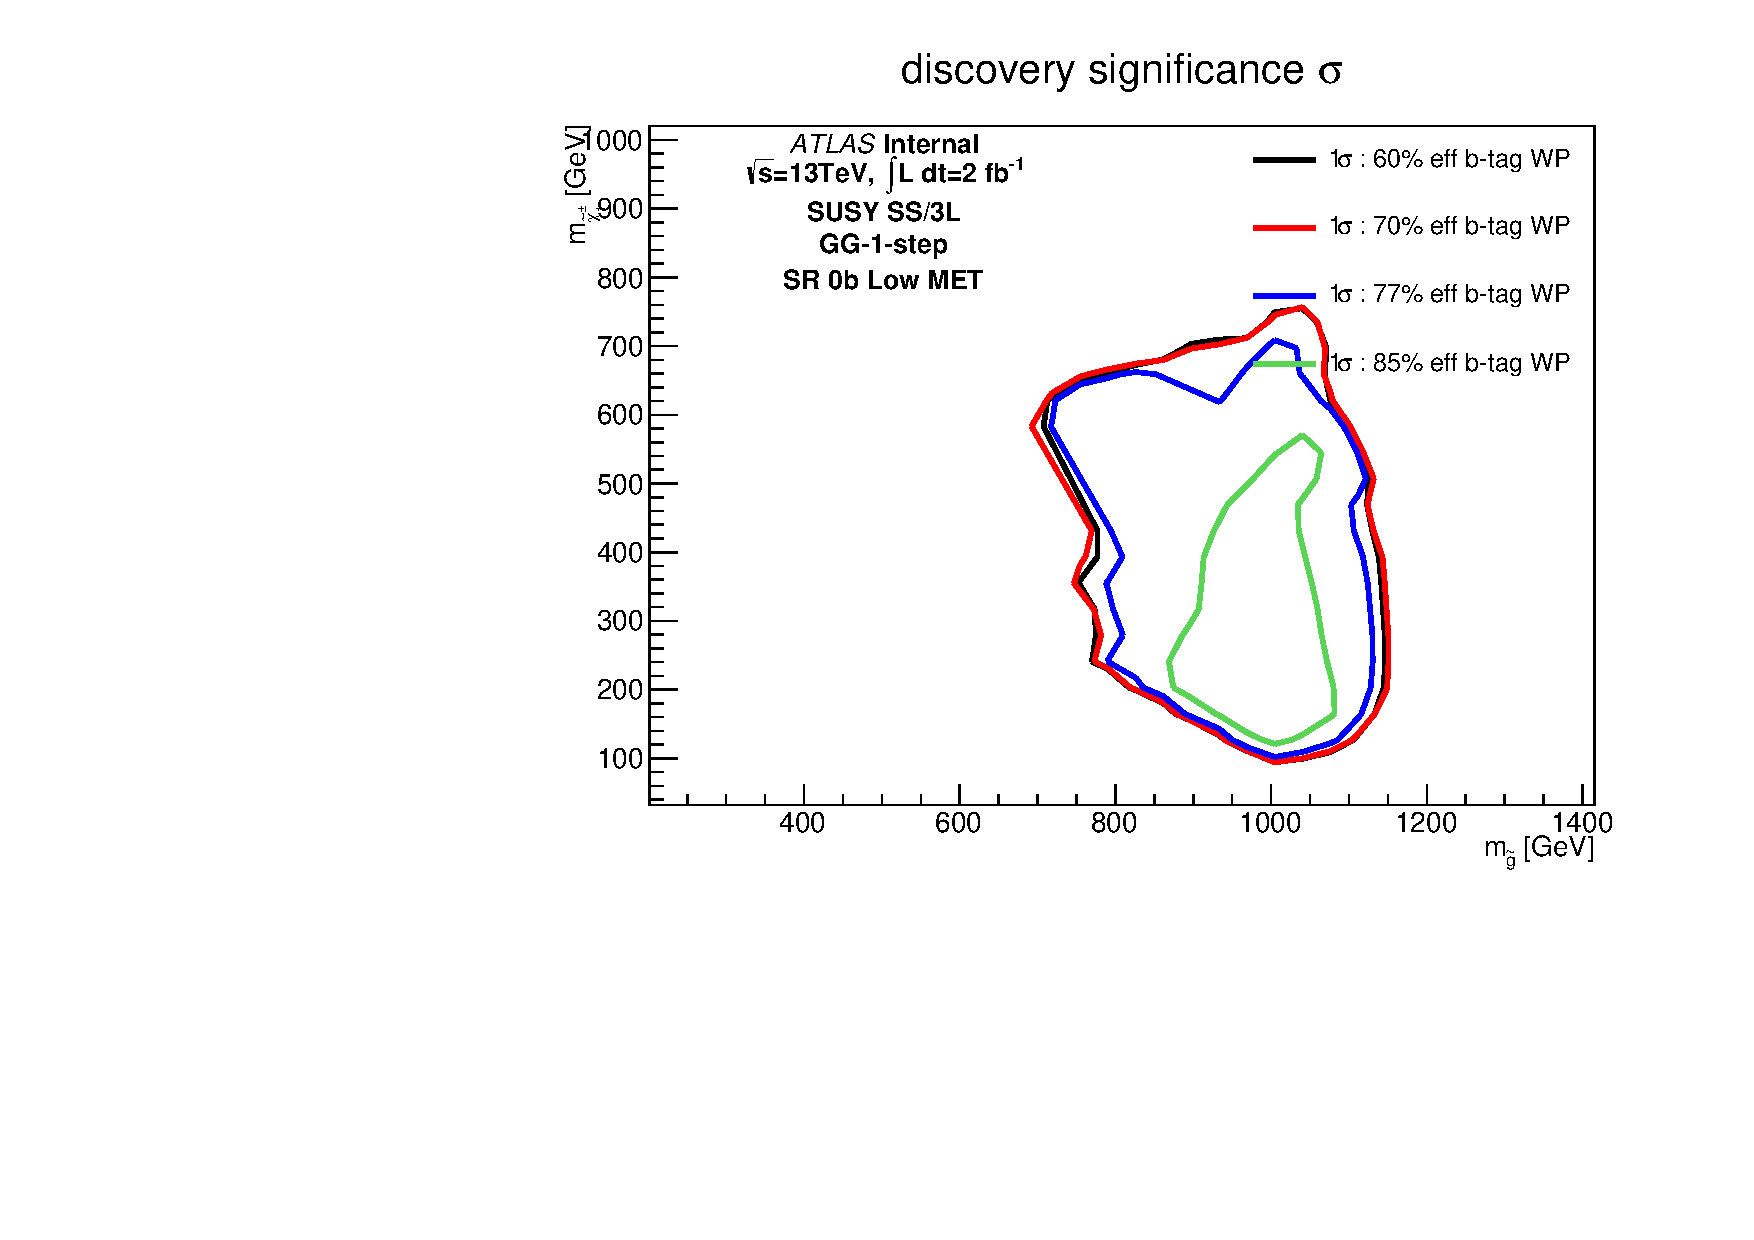
\includegraphics[width=0.45\textwidth]{FIGURES/BTAGGINGMC15/L2fb/plot_significance_gg1step_CutSR0BL60_all.pdf}        
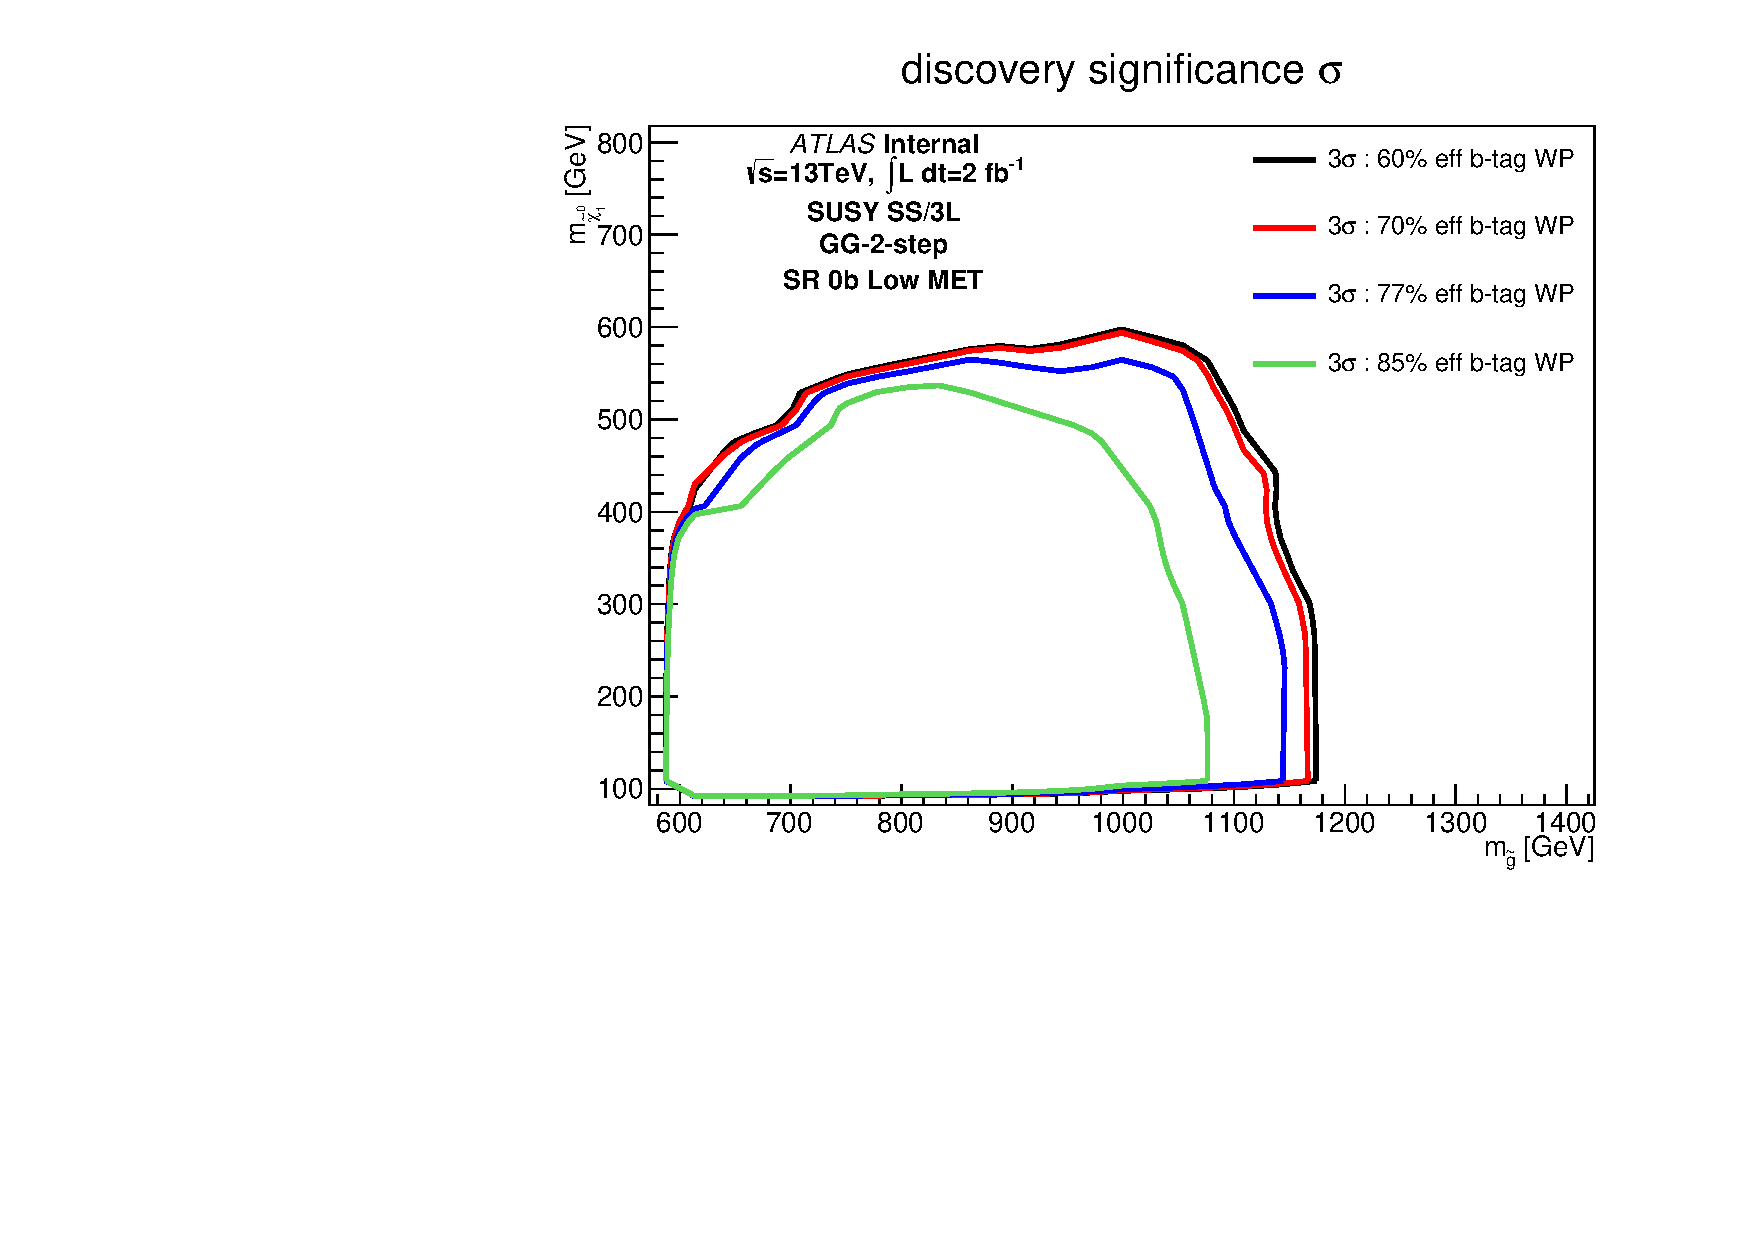
\includegraphics[width=0.45\textwidth]{FIGURES/BTAGGINGMC15/L2fb/plot_significance_gg2step_CutSR0BL60_all.pdf}          
\end{center}
\vspace{-0.2cm}
\caption{Gaussian discovery signal significance for the various signal-like regions where the different models are sensitive.
Three signal models are tested: the gluino-stop off-shell (top), the gluino production mediated by charginos (bottom left) and the 2-step gluinos via charginos (bottom right).
$b$-jet tagging efficiency working points supported by the heavy flavour working group are 60\%(black), 70\%(red), 77\%(blue) and 85\%(green).
Expectations are estimated assuming an integrated luminosity of 2~fb$^{-1}$ of 13~TeV.}
\label{fig:btaggingGrid}
\end{figure}

Figure~\ref{fig:btaggingGrid} shows the discovery signal significance using a simple Gaussian approximation ($S/\sqrt{S+(\Delta B)^2}$) for different choices of the $b$-tagging working point (60\%, 70\%, 77\% and 85\%) with a flat assumption on the background uncertainty of 40\%. The signal region for each of the models was chosen based on the highest sensitivity.
The 3$b$ Soft signal-like region was found to be the most performant for the gluino-stop off-shell production, 
and the 0$b$-5j signal-like region for the gluino production mediated by charginos as well as the 2-step 
gluino production mediated by gauginos. 
%As more signal simulations become available similar studies would be performed for sbottom direct production and gluinos (and squarks) 2-step models mediated via sleptons.
The 70\% $b$-tagging efficiency working point is chosen since it is the best compromise allowing to reach good sensitivity in the different tested signal models.

%Similar studies with detailed information comparing the performance of previous MV1 (rel-19) tagger and MV2c20 (rel-20) are shown in Appendix~\ref{app_btagging}.

\subsection{Leptons}
\label{sec:objects_leptons}

This section summarizes the electron and muon object selection, as well as developments done in the optimization of the
lepton isolation and electron acceptance cuts.

\subsubsection{Electrons}
\label{sec:objects_electrons}

The electron selection is summarized in Table~\ref{tab:lepdef}. The Egamma CP group recommends the likelihood-based electron identification~\cite{ATLAS-CONF-2014-032} for Run-2, since it provides a factor of two better background rejection than the cut-based identification.
Four working points ({\tt VeryLooseLH}, {\tt LooseLH}, {\tt MediumLH}, {\tt TightLH}) are available for LH electrons.

Pre-selected electrons must satisfy the {\tt LooseLH} requirements and have $E_\mathrm{T}>10$~GeV and $|\eta|<2.47$. 
Electrons in the LAr crack region ($1.37<|\eta|<1.52$) are rejected to reduce the contribution from non-prompt electrons. 
A requirement on the transverse impact parameter of $|d_0/\sigma(d_0)|<5$ (as recommended by TrackingCP) is also applied to pre-selected electrons and helps reducing the contribution from charge mis-identification. 
Signal electrons are additionally required to pass the isolation cuts defined in~\ref{sec:isolation} 
as well as the {\tt TightLH} identification criteria and standard requirements of the longitudinal impact parameter ($|z_0 \cdot sin(\theta)|<$ 0.5 mm, as recommended by TrackingCP).

A multiplicative event weight is applied for each signal electron in MC to the overall event weight 
in order to correct for differences in efficiency between data and MC as recommended by the Egamma group.

\subsubsection{Muons}
\label{sec:objects_muons}

The muon selection is summarized in Table~\ref{tab:lepdef}. The Run-2 muon reconstruction is performed by the so-called \textit{third chain}: 
it has been designed to combine the best features of the Run-1 STACO and MUID chains to provide the best performance. 
The following muon selection working points are supported:
{\tt Tight}, {\tt Medium}, {\tt Loose} and {\tt VeryLoose}. 

Pre-selected muon candidates must pass the {\tt Medium} muon quality cuts and have  $p_\mathrm{T} > 10\GeV$ and $|\eta| < 2.4$.
A smearing procedure is applied to the muon $p_\mathrm{T}$.  
A multiplicative event weight is applied for each selected muon in MC to the overall event weight in order to correct for differences in efficiency between data and MC as recommended by the Muon CP group. 

Finally, signal muon candidates are required to pass the isolation cuts defined in~\ref{sec:isolation} as well as the requirements on the impact parameter of $|d_0/\sigma(d_0)|<3$ and $|z_0 \cdot sin(\theta)|<$ 0.5 mm, as recommended by TrackingCP.


Note that events with ``cosmic'' muons, or ``Bad'' muon are vetoed as described in Section~\ref{sec:presel}.


%%%%%%%%%%%%%%%%%%%%%%%%%%%%%%%%%%%%%%%%%%%%%%%%%%%%%%%%%%%%%
\begin{table}[htb!]
\caption{Summary of the electron and muon selection criteria. The signal
  selection requirements are applied on top of the preselection. The
  lepton-jet isolation requirement is applied after electron-jet overlap
  removal.}
\label{tab:lepdef}
\begin{center}
    \begin{tabular}{|l|c|c|}
      \hline
      \hline
       & \textbf{Pre-selected Electron} & \textbf{Pre-selected Muon} \\
      \hline
      \hline
      Acceptance     & $\pt > 10\,\GeV, |\eta^\mathrm{clust}| < 2.47$  & $\pt > 10\,\GeV, |\eta| < 2.5$ \\
                     &  except $1.37<|\eta^\mathrm{clust}|<1.52$       & \\
      \hline
      Quality & {\tt LooseLLH} & {\tt{xAOD::Muon::Medium}} \\
%      \hline
%      Impact parameter &  $|d_0/\sigma(d_0)|<$ 5.0 & - \\
      \hline
      $\ell$-jet Isolation      & $\Delta{}R(e,jet)$~$>$~0.4 & $\Delta{}R(\mu,jet)$~$>$~0.4 \\
      \hline
      Impact parameter & $|d_0/\sigma(d_0)|<5.0$  & \\
      \hline\hline
       & \textbf{Signal Electron} & \textbf{Signal Muon} \\
      \hline
      \hline
      Quality & {\tt TightLLH} & -\\
       & $|\eta|<2.0$  & -\\
            \hline
      Isolation                & ``FixedCutTight '' & ``FixedCutTightTrackOnly'' \\
      \hline
      Impact parameter & $|z_0 \cdot sin(\theta)|<$ 0.5 mm   & $|z_0 \cdot sin(\theta)|<$ 0.5 mm \\ 
                       &                                     & $|d_0/\sigma(d_0)| < 3.0$\\
     \hline
\end{tabular}
\end{center}
\end{table}
%%%%%%%%%%%%%%%%%%%%%%%%%%%%%%%%%%%%%%%%%%%%%%%%%%%%%%%%%%%%


\subsubsection{Lepton isolation}
\label{sec:isolation}

The isolation working points proposed from this analysis were accepted by the ATLAS Isolation forum and implemented as officially supported working points in the {\tt IsolationSelectionTool}. Unless otherwise stated, the following isolation working points are used in the analysis:
\begin{itemize}
\item Electrons: {\tt TightLLH}, ptvarcone20/\pt$<$0.06 and topoetcone20/\pt$<$0.06 (``FixedCutTight'')
\item Muons: ptvarcone30/\pt\ $<0.06$ (``FixedCutTightTrackOnly'')
\end{itemize}
%Note that no isolation scale factors are used so far in the analysis, but will be released by the EGamma and Muon combined performance groups with the whole 2015 dataset.
Isolation scale factors determined by the CP groups for these working points are applied. 

More details on the isolation studies performed in the context of this analysis can be found in Appendix~\ref{app:iso}.



\subsubsection{Electron acceptance}
\label{sec:eleAcceptance}

Dedicated studies have been conducted to evaluate the impact of a reduction of the $|\eta|$ coverage for electrons. 
This is motivated by the fact that the largest contributions from charge-flip and fake lepton backgrounds 
are observed at $|\eta|>2$ and in the LAr crack region ($1.37<|\eta|<1.52$), 
due to poorer detector resolution or increased amount of material in these regions. 

Table~\ref{tab:eleEta} shows the impact on the expected event yields when reducing the electron $|\eta|$ acceptance 
for the two leading electrons (taking a reference the case of $|\eta|<2.3$). The event selection applied to compute those numbers 
requires SS/3L, at least 3 jets with $\pt > 30$~GeV and $m_{ee}$ outside the 84-98~GeV range to reduce the contribution 
from charge flips. 

%%%%%%%%%%%%%%%%%%%%%%%%%%%%%%%%%%%%%%%%%%%%%%%%%%%%%%%%%%%%%
\begin{table}[htb]
\caption{Relative decrease in the event yield when reducing the $|\eta|$ acceptance for the two leading electrons with respect to $|\eta|<2.3$. The reference is considered to be $|\eta|$~$<$~2.47, and the crack region is excluded in all the cases. Numbers are shown for the event selection described in the text and separately for events with 1 or more $b$-jets.}
\label{tab:eleEta}
\begin{center}
    \begin{tabular}{|l|c|c|c|c|c|} \hline
                   & Prompt SS & $\ttbar +W$ & Gtt (G900\_L100) & Non-prompt leptons & Charge flip \\ \hline\hline
==1$b$, $|\eta|<1.37$ & 14\% & 16\% & 12\%  & 28\% & 69\% \\
==1$b$, $|\eta|<2.0$  & 5.4\%  & 6\%  & 7\%&  11\% & 37\% \\ 
==1$b$, $|\eta|<2.3$  & 0.4\%  & 1.5\%  & 4.7\%&  3.6\% &  11\% \\ \hline
$>$1$b$, $|\eta|<1.37$ & 13\% & 18\% & 10\%  & 44\% & 66\% \\
$>$1$b$, $|\eta|<2.0$  & 4.3\%  & 6.5\%  & 2.9\%&  21\% &  30\% \\ 
$>$1$b$, $|\eta|<2.3$  & 1.3\%  & 1.5\%  & 0.3\%&  8\% &  5.8\% \\  \hline
\end{tabular}
\end{center}
\end{table}
%%%%%%%%%%%%%%%%%%%%%%%%%%%%%%%%%%%%%%%%%%%%%%%%%%%%%%%%%%%%

As shown, reducing the acceptance to $|\eta|<2.0$ would reduce the contribution from processes with prompt 
SS/3L by 6.5\% or less, but the reduction in non-prompt leptons (11-21\%) and charge flip (30-37\%) is quite larger. 
Reducing the acceptance more severely for the two leading electrons to $|\eta|<1.37$ would reduce the non-prompt and 
charge flip components by 28-44\% and $\sim$69\%, respectively, with a reduction of only 13-18\% for prompt SS/3L processes. 

Therefore, this study proves that additional rejection against some of the main backgrounds affecting the analysis can be achieved 
by reducing the $|\eta|$ acceptance of the electrons. 
As illustrated in Table~\ref{tab:lepdef} we chose in conclusion to reject electrons with $|\eta|>2.0$ or in the EM calorimeter cracks ($1.37<|\eta_\text{cluster}|<1.52$). 
Note that these requirements are applied to electrons regardless of the lepton multiplicity of the event.

\subsection{Overlap removal}
\label{sec:objects_overlap_removal}

According to the above definitions, one single final state object may fall in more than one category, being therefore effectively double-counted. 
For example, one isolated electron is typically reconstructed both as an electron and as a jet. A procedure to remove overlaps between final state objects was therefore put in place, and applied on pre-selected objects. 
For this iteration, recommendations from the Harmonization effort~\cite{Harmonization} have been fully adopted. 
%The only exception is the usage a narrower cone for the muon-jet overlap removal (0.2 instead of 0.4).
%A gain of a few \% on signal acceptance and background rejection was observed with respect to the previous overlap-removal definitions, where no $b$-jet information, neither jet-track counting was used.
%The small gain is more evident on the muon channels, with up to 9\% higher acceptance for a Gtt sample, more details can be found in the appendix~\ref{app_overlapremoval} 

The procedure performed is described as follows:

\begin{itemize}

\item First, jets that are angularly close (cone of $\Delta R_y < 0.2$, note the usage of rapidity instead of pseudo-rapidity) 
to a pre-selected (non-isolated) electron are removed from the jet list, 
except if the $b$-tagging weight satisfies the 80\% working point (the electron is then likely coming from a semileptonic $b$-quark decay, so it is removed and the jet is kept). 
%Otherwise both the electron and the jet are kept. 

\item Following this, pre-selected electrons are removed if their distance to the closest jet is $\Delta R_y < 0.4$. 
Then if the $\Delta R_y$ between a jet and a muon is less than 0.4, 
one looks at the number of tracks associated to the jet ({\tt xAOD::JetAttribute::NumTrkPt500}): 
if strictly less than 3 the jet is removed (and the muon is kept),  
otherwise the muon is removed (and the jet is kept).
 
\item If there are an electron and a muon with $\Delta R_y<0.01$, the former is likely to originate from a bremsstrahlung 
of the muon. Such a muon momentum is not measured correctly so that in this case, both the electron
and the muon are removed.

\item Finally, if there are two electrons with $\Delta R_y<0.05$,  the electron with the highest \pT is kept and the other one is discarded.

\end{itemize}

Note that preliminary studies with DC14 data showed a few percent gain in sensitivity if using a narrower cone for the muon-jet overlap removal ($\Delta R_y<0.2$), 
but this was found to introduce features in the muon real and fake efficiency used in the matrix method (see Appendix~\ref{App:RealEfficiency}). 
Therefore, for simplicity and robustness in the analysis, it was decided to used the default value of $\Delta R_y<0.4$. 

%If the distance between two electrons is $\Delta R<0.1$, it is most likely to be that two
%tracks are associated with one calorimeter cluster mistakenly. In this case, lower $E_{\rm T}$ electron 
%is removed. Also 
% OLD TEXT:
%If there are an electron and muon with $\Delta R<0.1$, it is likely to be the bremsstrahlung
%of the muon, and it is therefore removed.

%Studies supporting the update to the latest recommendations (and choice of narrower cone mentioned above) are described below.
%
%Since signal samples in MC15 were not available at the time the study was performed, DC14 samples (signal and background) were used.
%Various signals models were used (Gtt 1300~GeV, $\tilde{\chi_0}$=100~GeV, Gtt 1300~GeV, $\tilde{\chi^0_1}$=700~GeV, sbottom 1300~TeV, 2-step (gluino) 700,400GeV) 
%to obtain significance estimates for different cone-distance used in the overlap-removal between jets and muons.
%Figure~\ref{fig:OR_significance} show the significance (using a Poissonian estimator) for the various flavour channels as well as their combination, after full event selection requirements.
% 
%\begin{figure}[htb!!]
%\begin{center}
%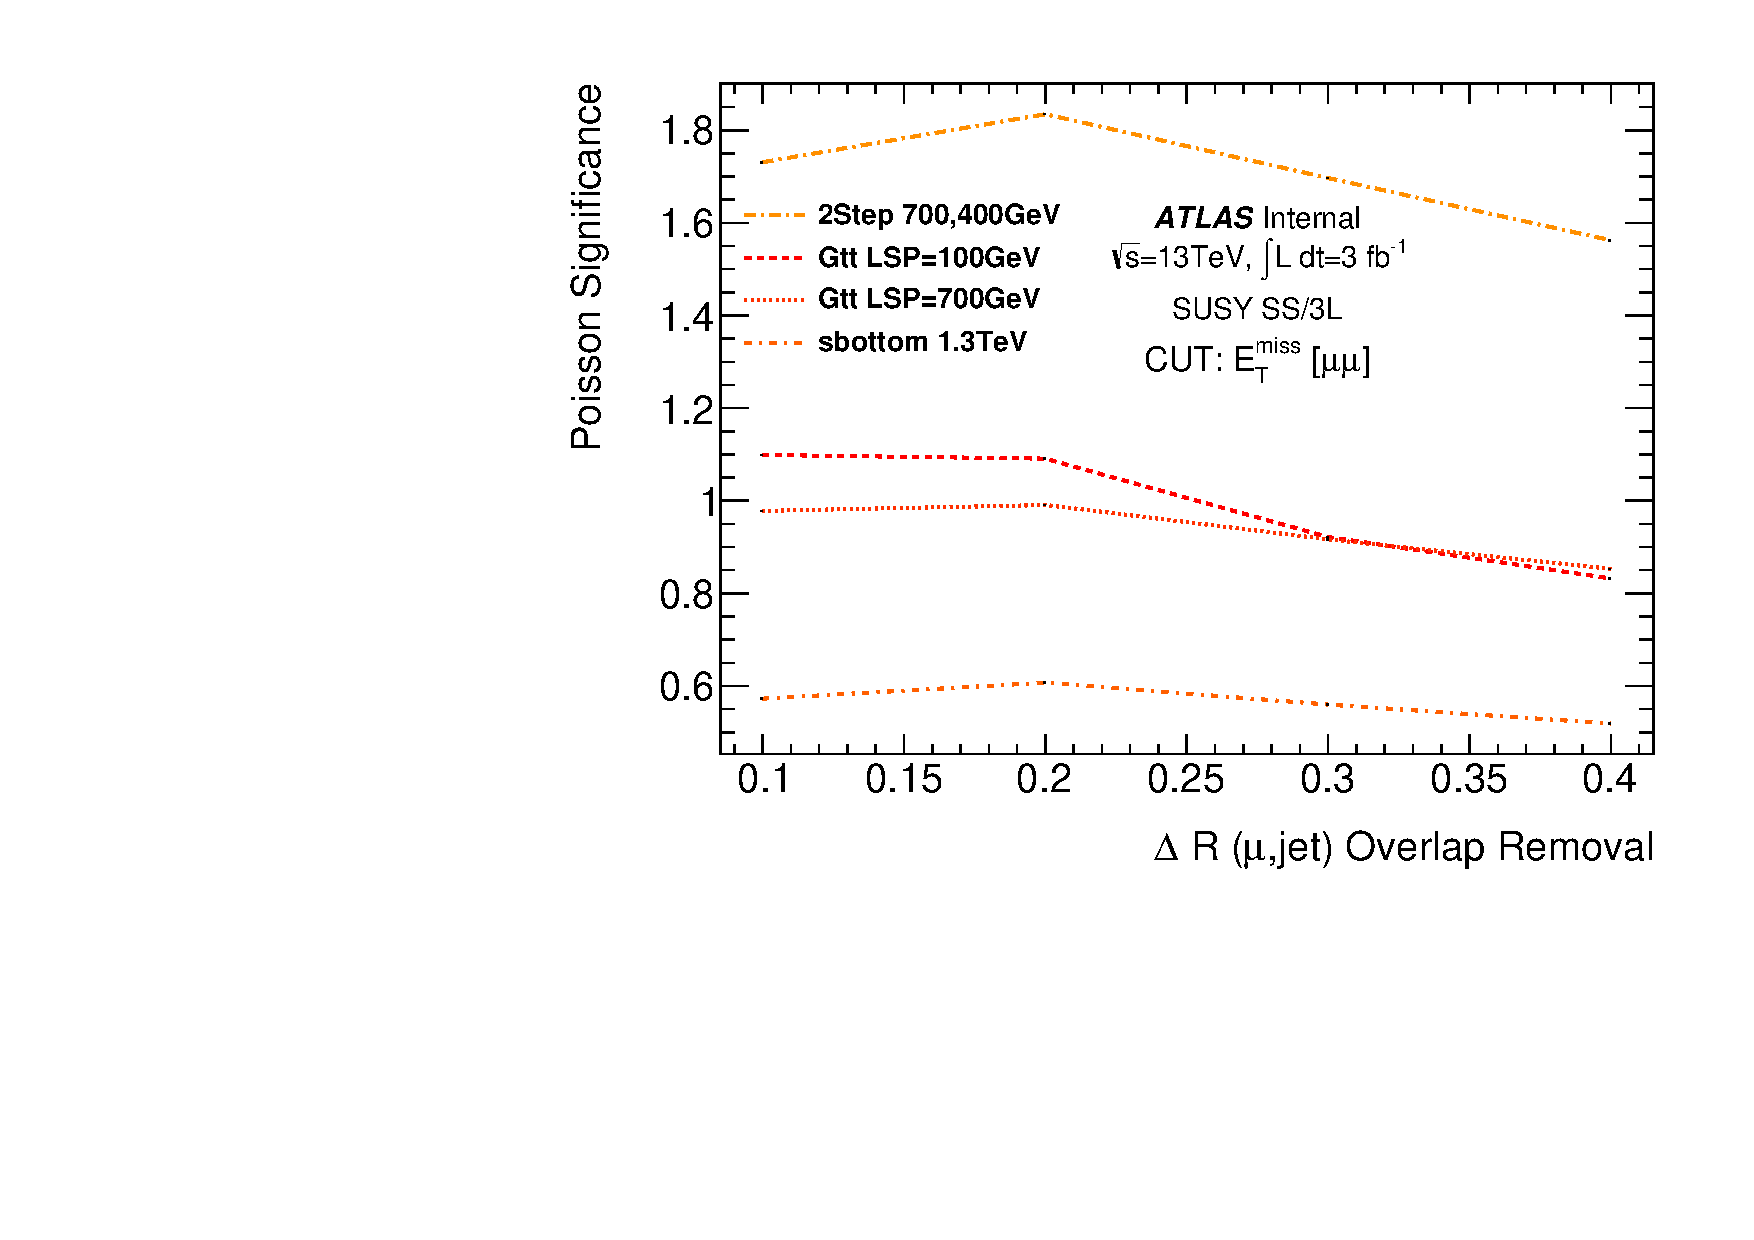
\includegraphics[width=0.45\textwidth]{OVERLAPREMOVAL/plot_significance_mm.pdf} 
%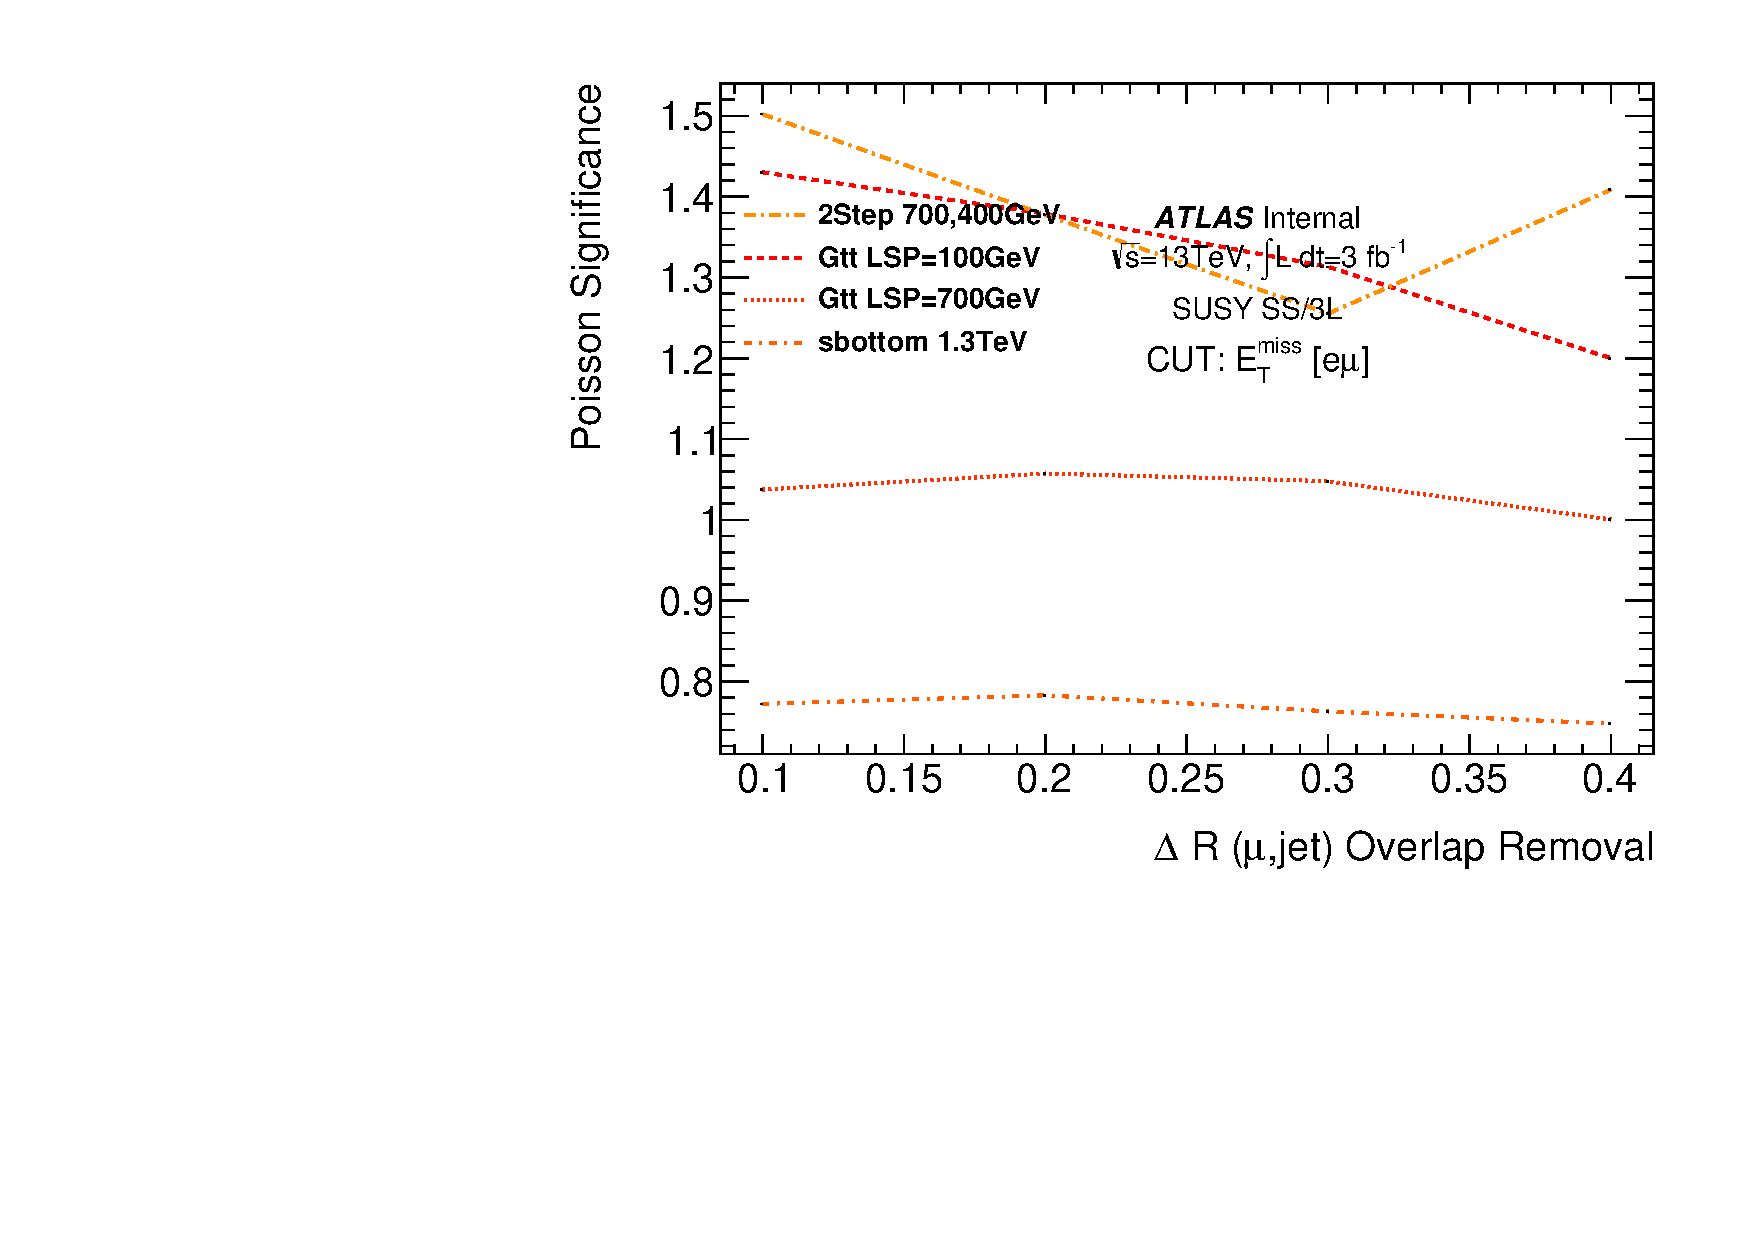
\includegraphics[width=0.45\textwidth]{OVERLAPREMOVAL/plot_significance_em.pdf} 
%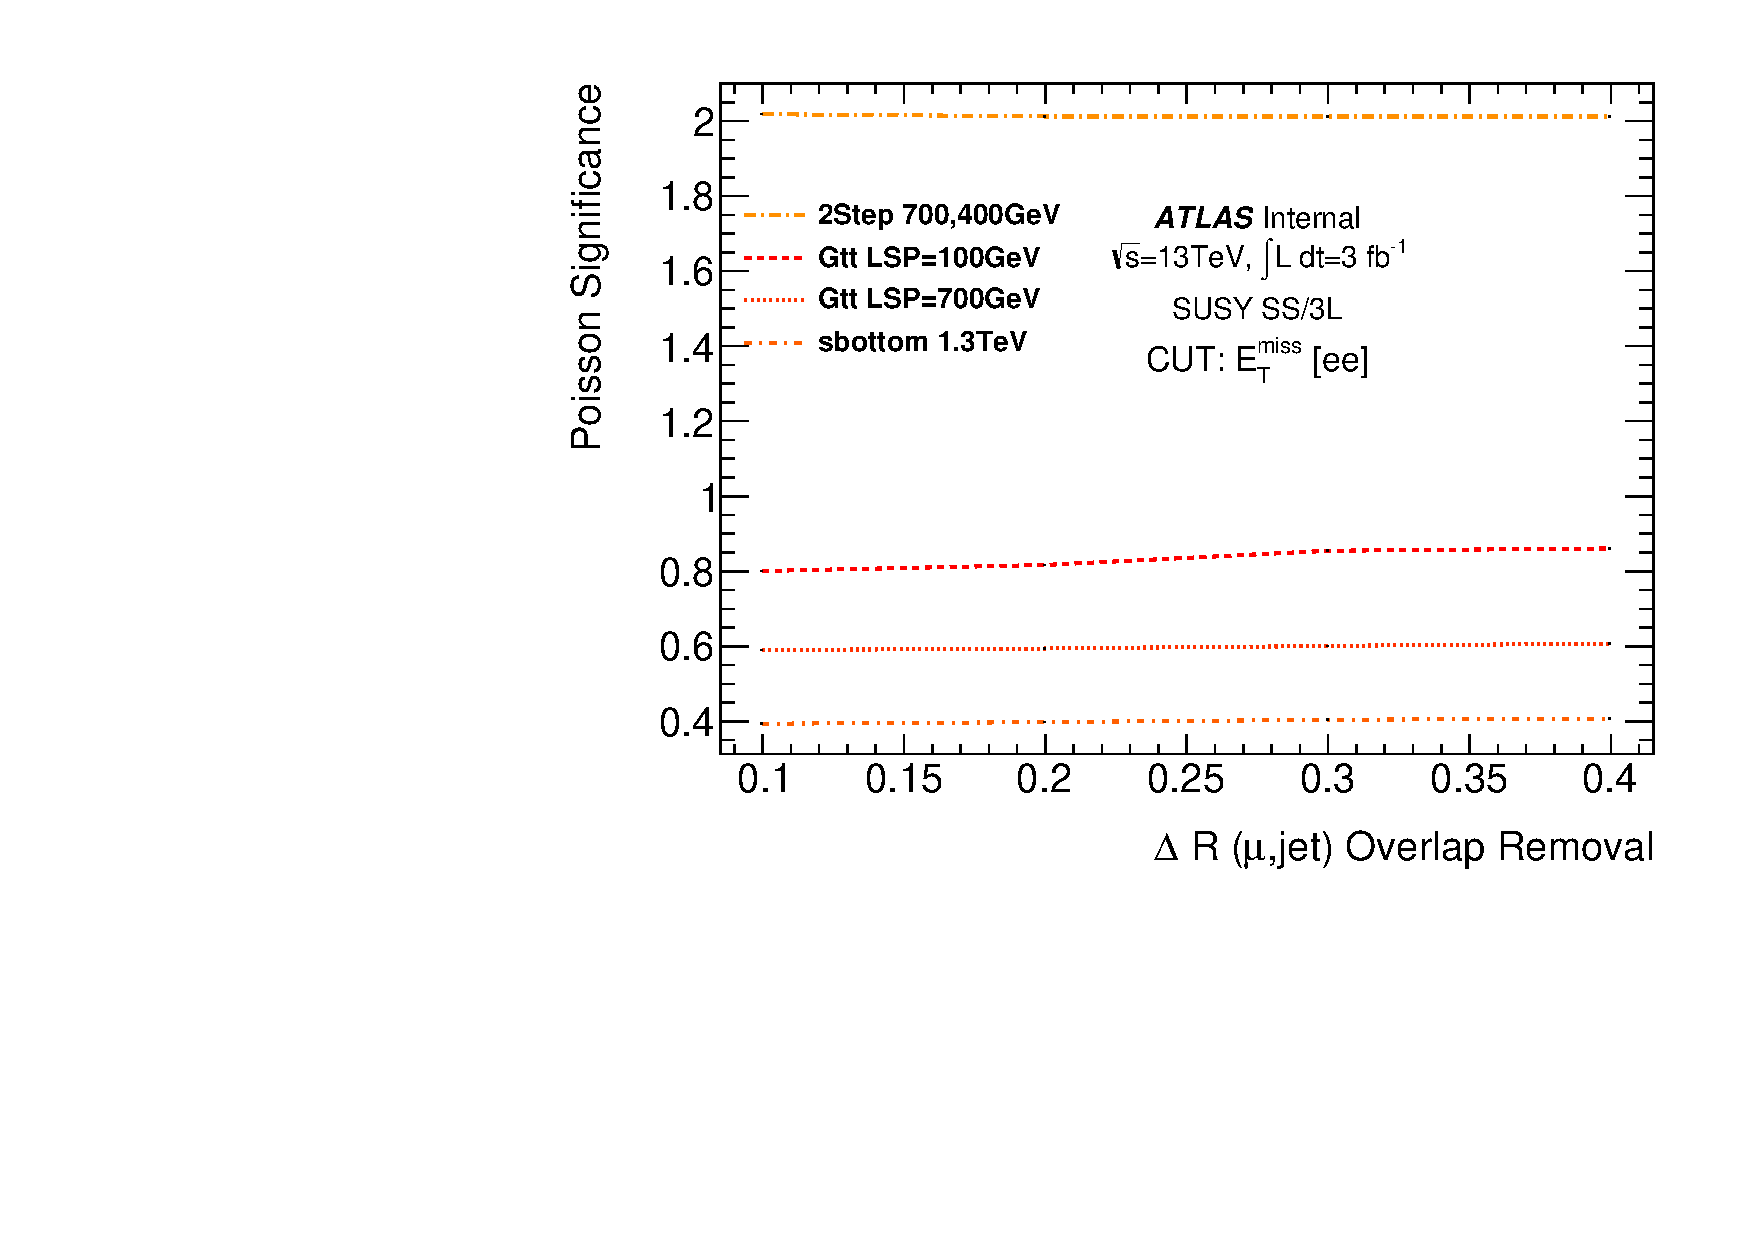
\includegraphics[width=0.45\textwidth]{OVERLAPREMOVAL/plot_significance_ee.pdf} 
%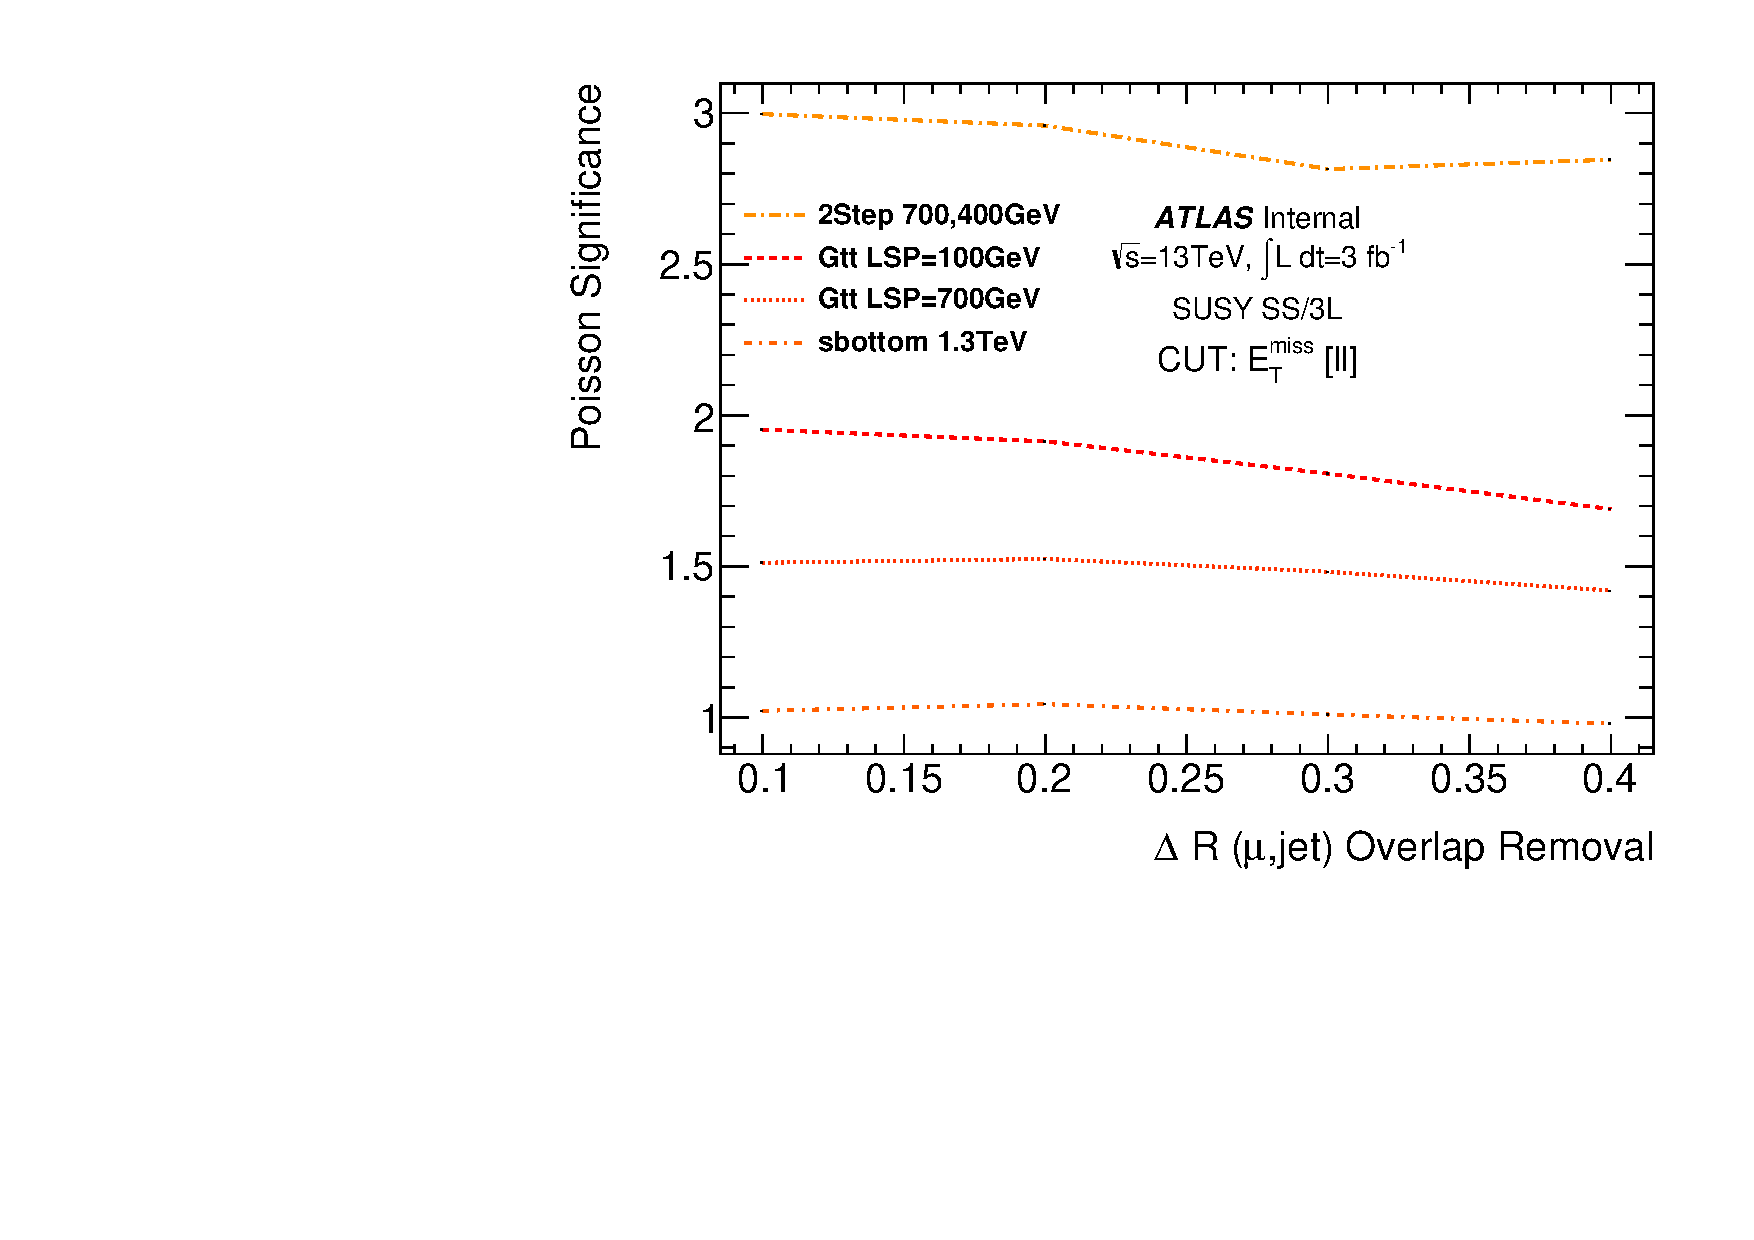
\includegraphics[width=0.45\textwidth]{OVERLAPREMOVAL/plot_significance_ll.pdf} 
%\end{center}
%\vspace{-0.2cm}
%\caption{Discovery significance for an assumed integrated luminosity of 3~fb$^{-1}$, for different choices of cone separation used for the muon-jet object overlap removal in various signal models. 
%Top figures display the significance for the muon-related channels ($\mu\mu$ and $e\mu$) and bottom figues illustrate the effect on the $ee$ channel as well as the flavour combination.}
%\label{fig:OR_significance}
%\end{figure}
%
%The studies seem to favor a choice of a $\Delta R$ of 0.2.  


\subsection{Missing transverse energy}
\label{sec:objects_met}

The missing transverse energy (\met) is rebuilt using the xAOD container ``MET\_RefFinal'' as input and using the calibrated electron, muon and jet objects 
(and baseline photons according to SUSYTools definitions). 
In this version of the analysis, the track soft term is used for building the \met\ following the defaults in SUSYTools-00-07-17.


\subsection{Lepton truth matching}
\label{sec:truth_matching}

In several studies presented in this document, 
a lepton truth matching strategy is applied to distinguish the lepton originating from prompt decays of gauge boson or SUSY particles 
from non-prompt leptons originating from semileptonic $b$-decays, photon conversions or fakes. 
This strategy largely relies on the information from the {\tt MCTruthClassifier} tool. 
However, the latter does not always allow to properly classify electrons originating from a photon conversion, 
where it is important to fully understand the origin of the photon and its possible proximity to a prompt electron 
(FSR, brehmsstrahlung, which is the main mechanism leading to charge-flip electrons). 
In these cases, we complete this information by a matching within a cone of $\Delta R <0.1$ with truth prompt electrons, 
which are identified as the decays of heavy bosons ($W$, $Z$, $h$) or SUSY particles. 
This is however only possible in MC generators storing intermediate resonances in the event record, 
i.e. notably MC samples in which decay chains are handled by Pythia. 

\FloatBarrier

